% ---------------------------------------------------------------------------
% Shared preamble for the two-point lock-in master reference.
% ---------------------------------------------------------------------------
\documentclass[11pt,a4paper]{report}

\usepackage[T1]{fontenc}
\usepackage[utf8]{inputenc}
\usepackage{lmodern}
\usepackage{microtype}
\usepackage[margin=2.4cm,top=2.6cm,bottom=2.6cm]{geometry}
\usepackage{graphicx}
\usepackage{booktabs}
\usepackage{longtable}
\usepackage{array}
\usepackage{amsmath}
\usepackage{amssymb}
\usepackage{siunitx}
\usepackage{xcolor}
\usepackage[most]{tcolorbox}
\usepackage{enumitem}
\usepackage{titlesec}
\usepackage{fancyhdr}
\usepackage{caption}
\usepackage{float}
\usepackage{underscore}          % lets _ work in text mode; keeps identifiers readable
\usepackage[hidelinks,bookmarksnumbered]{hyperref}

\sisetup{detect-weight=true,detect-family=true}

% --- colours -------------------------------------------------------------
\definecolor{accent}{HTML}{1F4E79}
\definecolor{good}{HTML}{1B7A3D}
\definecolor{bad}{HTML}{A81E1E}
\definecolor{warn}{HTML}{B36B00}
\definecolor{rulegrey}{HTML}{888888}
\definecolor{shade}{HTML}{F2F5F8}

% --- headings ------------------------------------------------------------
\titleformat{\chapter}[display]
  {\normalfont\huge\bfseries\color{accent}}{\Large\chaptertitlename\ \thechapter}{8pt}{\Huge}
\titlespacing*{\chapter}{0pt}{-18pt}{22pt}
\titleformat{\section}{\normalfont\Large\bfseries\color{accent}}{\thesection}{0.7em}{}
\titleformat{\subsection}{\normalfont\large\bfseries}{\thesubsection}{0.7em}{}
\titleformat{\subsubsection}{\normalfont\normalsize\bfseries}{\thesubsubsection}{0.7em}{}

\setcounter{tocdepth}{2}
\setcounter{secnumdepth}{3}

\pagestyle{fancy}
\fancyhf{}
\fancyhead[L]{\small\color{rulegrey}Two-point lock-in --- master reference}
\fancyhead[R]{\small\color{rulegrey}\thepage}
\renewcommand{\headrulewidth}{0.4pt}

\setlist{itemsep=2pt,topsep=4pt,parsep=0pt}

% --- semantic macros -----------------------------------------------------
\newcommand{\co}[1]{\texttt{\small #1}}
\newcommand{\file}[1]{\texttt{\small #1}}
\newcommand{\us}{\si{\micro\second}}
\newcommand{\ms}{\si{\milli\second}}
\newcommand{\nTrtHz}{\si{\nano\tesla\per\sqrt{\hertz}}}
\newcommand{\etaunit}{nT/$\sqrt{\text{Hz}}$}
\newcommand{\tauro}{$\tau$}

\newcommand{\Done}{\textcolor{good}{\textbf{DONE}}}
\newcommand{\Open}{\textcolor{bad}{\textbf{OPEN}}}
\newcommand{\Partial}{\textcolor{warn}{\textbf{PARTIAL}}}

% Callout boxes
\newtcolorbox{keybox}[1][]{colback=shade,colframe=accent,coltitle=white,
  fonttitle=\bfseries,title={#1},boxrule=0.9pt,arc=2pt,left=6pt,right=6pt,
  top=5pt,bottom=5pt,breakable}
\newtcolorbox{retractbox}[1][]{colback=bad!5,colframe=bad,coltitle=white,
  fonttitle=\bfseries,title={#1},boxrule=0.9pt,arc=2pt,left=6pt,right=6pt,
  top=5pt,bottom=5pt,breakable}
\newtcolorbox{openbox}[1][]{colback=warn!6,colframe=warn,coltitle=white,
  fonttitle=\bfseries,title={#1},boxrule=0.9pt,arc=2pt,left=6pt,right=6pt,
  top=5pt,bottom=5pt,breakable}

% Table helpers
\newcommand{\hd}[1]{\textbf{#1}}
\newcommand{\tstrut}{\rule{0pt}{2.5ex}}


\begin{document}

% ------------------------------------------------------------------ title
\begin{titlepage}
\centering
\vspace*{2.4cm}
{\Huge\bfseries\color{accent} Two-Point Parked Lock-In\par}
\vspace{0.5cm}
{\LARGE\color{accent} Master Reference\par}
\vspace{1.1cm}
{\large Acquisition methods $\cdot$ timing breakdown $\cdot$ sensitivity\\
open defects $\cdot$ work log\par}
\vspace{2.0cm}

\begin{minipage}{0.82\textwidth}
\small
\raggedright
\textbf{Project} \quad NV compact magnetometer, RFSoC4x2 + QICK-DAWG\\
\textbf{Repository} \quad \file{nv_magnetometer_project}, branch \co{main}\\
\textbf{Sessions covered} \quad 2026-08-04, 2026-08-06, 2026-08-14\\
\textbf{Written} \quad 2026-08-17\\[0.7em]
\textbf{Supersedes} \quad
\file{docs/2026-08-06_twopoint_timing/TIMING_AND_NOISE_ANALYSIS.md} and
\file{docs/2026-08-14_twopoint_methods/TWOPOINT_METHODS_AND_TIMING.md},
both of which remain in the repository as the record of what was believed when.
Chapter~\ref{ch:retractions} lists every disagreement.\\[0.7em]
\textbf{Regenerate every number} \quad \co{python scripts/analyze_twopoint_0814.py}
\end{minipage}

\vfill

\begin{minipage}{0.82\textwidth}
\begin{keybox}[The three findings, in one paragraph each]
\small
\textbf{Rate.} An \co{acquire()} call costs 10--11.4\,ms of host round-trip whatever
the program does, and the FPGA work runs underneath it. Halving the readout window
cut the FPGA work by 4$\times$ and changed the rate by 0.4\%. The averaged mode
therefore sits at $\sim$88\,Hz at any setting, and averaging is \emph{free} up to the
call floor.

\textbf{Sensitivity.} The reference-photodiode fix bought \textbf{4.1$\times$}: the
burst-mode noise floor went from 158 to \textbf{38\,\etaunit}. Burst is the best
operating point available today.

\textbf{Bandwidth.} Streaming delivers \textbf{1041.7\,Hz} with a gapless,
duplicate-free rep axis --- the 1\,kHz target is met. Its noise floor is
$\sim$6$\times$ the burst floor for reasons not yet identified, which is the single
highest-value open item.
\end{keybox}
\end{minipage}

\vspace{1.2cm}
{\small\color{rulegrey} Chalach Kasemtantikul\par}
\end{titlepage}

% ------------------------------------------------------------------ contents
\tableofcontents
\clearpage

% ------------------------------------------------------------------ body
\chapter{How to read this document}

\section{What this is}

This is the single reference for the two-point parked-frequency lock-in on the
NV compact magnetometer: how each acquisition method works, exactly where the
acquisition time goes, what sensitivity each method delivers, which defects are
open, and what has been changed in the code so far.

It merges and supersedes two earlier documents:

\begin{itemize}
  \item \file{docs/2026-08-06\_twopoint\_timing/TIMING\_AND\_NOISE\_ANALYSIS.md}
        --- the 2026-08-06 session: timing budget, readout-window optimum,
        discovery of the burst-mode replay.
  \item \file{docs/2026-08-14\_twopoint\_methods/TWOPOINT\_METHODS\_AND\_TIMING.md}
        --- the 2026-08-14 session: the three modes compared, the per-call floor,
        two open defects.
\end{itemize}

Both remain in the repository as the record of what was believed when. Where they
disagree with this document, this document wins, and
Chapter~\ref{ch:retractions} lists every such disagreement explicitly.

\section{Where the numbers come from}

Every measured value here is regenerated by one script from committed CSV files:

\begin{center}
\co{python scripts/analyze\_twopoint\_0814.py}
\end{center}

It writes \file{docs/2026-08-14\_twopoint\_methods/tables/*.csv} and
\file{figures/*.png}; this document quotes those tables. Nothing is hand-typed,
so re-running the script after a new session refreshes the numbers rather than
invalidating them. Values that can only be measured on the rig are marked
\Open{} and named as such --- there are five of them, all in
Chapter~\ref{ch:todo}.

\section{The three findings that matter most}

\begin{keybox}[1. The acquisition rate is set by the host, not by the readout window]
An \co{acquire()} call costs \textbf{10--11.4\,ms of host round-trip whatever the
program does}, and the FPGA pulse work runs \emph{underneath} that rather than
adding to it. Halving the readout window from \SI{213}{\micro\second} to
\SI{120}{\micro\second} cut the FPGA work from 9.80\,ms to 2.40\,ms and changed
the rate by nothing (87.5 $\rightarrow$ 86.8\,Hz).

Consequences: shortening $\tau$ is not a rate lever in averaged mode; averaging
more reps is \emph{free} up to the call floor; and beating $\sim$90\,Hz requires
amortising the call across many samples, which is what burst and streaming do.
See Chapter~\ref{ch:timing}.
\end{keybox}

\begin{keybox}[2. The photodiode fix bought 4.1$\times$, and burst mode shows it]
After the reference-photodiode gain was corrected and the signal diode stopped
saturating, the burst-mode noise floor went from \textbf{158 to 38\,\etaunit} ---
a factor of 4.1 at the same two parked points. Burst is the best operating point
available today by a wide margin. See Chapter~\ref{ch:sensitivity}.
\end{keybox}

\begin{keybox}[3. Streaming reaches 1\,kHz, but its noise floor is $\sim$6$\times$ burst]
Streaming delivered \textbf{1041.7\,Hz} with a gapless, duplicate-free rep axis
across 125\,000 reps --- the 1\,kHz target is met. Its noise floor, however, sits
a flat $\sim$6$\times$ above burst across 10--500\,Hz for reasons not yet
identified. Chapter~\ref{ch:defects} lists what has been ruled out and the
one-minute rig test that decides it.
\end{keybox}

\section{Status at a glance}

\begin{center}
\small
\begin{tabular}{@{}llll@{}}
\toprule
\hd{Item} & \hd{State} & \hd{Number} & \hd{Where} \\
\midrule
Averaged mode rate            & \Done    & 86.8--88.8\,Hz          & \S\ref{sec:avg} \\
Burst mode rate               & \Done    & 4167\,Hz in-burst       & \S\ref{sec:burst} \\
Streaming rate                & \Done    & 1041.7\,Hz              & \S\ref{sec:stream} \\
Best measured noise floor     & \Done    & 38\,\etaunit\ (burst)   & \S\ref{sec:etameas} \\
Readout window chosen         & \Done    & \SI{120}{\micro\second} & \S\ref{sec:window} \\
Timing model                  & \Done    & $\max(\text{host},\text{FPGA})$ & \S\ref{sec:model} \\
Free averaging implemented    & \Done    & 42 reps fit, 10 used    & \S\ref{sec:freeavg} \\
Per-mode post-processing      & \Done    & 3 pipelines             & \S\ref{sec:postproc} \\
Notebook reorganised          & \Done    & 4A/4B/4C + 5A/5B/5C     & \S\ref{sec:notebook} \\
\midrule
Burst replay root cause       & \Open    & 49.9\% of batches       & \S\ref{sec:replay} \\
Streaming noise excess        & \Open    & $\sim$6$\times$ burst   & \S\ref{sec:streamnoise} \\
Per-acquire noise term        & \Open    & does not average down   & \S\ref{sec:notshot} \\
ABBA ordering benefit         & \Open    & never tested on hardware & \S\ref{sec:abba} \\
Calibrated system sensitivity & \Open    & no field reference yet  & \S\ref{sec:notaclaim} \\
\bottomrule
\end{tabular}
\end{center}


\chapter{The measurement, from photons to \texorpdfstring{$\Delta f$}{delta f}}
\label{ch:estimator}

Before any timing discussion, this is what a ``sample'' actually is. All three
acquisition methods produce the same quantity by the same arithmetic; they differ
only in how many FPGA repetitions go into one sample and how the host collects
them.

\section{Two parked frequencies on one flank pair}

A single ODMR resonance is fitted (Lorentzian, from the Step~1 reference sweep),
giving its centre $f_0$, half-width $\gamma$, baseline $B$, and the two
maximum-slope points $f_-$ and $f_+$ on either flank. Rather than sweeping, the
microwave source is \emph{parked} alternately at $f_-$ and $f_+$ and the
photoluminescence is read at each.

\begin{align}
z_\pm &= \frac{\text{counts at } f_\pm}{\text{normalisation}}
   &&\text{normalised PL at each parked point} \\
L &= z_+ - z_-  &&\text{the lock-in signal} \\
\Delta f &= \frac{L - (b_+ - b_-)}{m_- - m_+}
   &&\text{shift of the resonance, in MHz}
\end{align}

where $b_\pm$ are the calibration baselines at the parked points and $m_\pm$ the
flank slopes, both measured off the reference sweep. Field is then
$\Delta B = \Delta f / \gamma_\text{NV}$ with
$\gamma_\text{NV} = \SI{28.024}{\kilo\hertz\per\micro\tesla}$ along the tracked
NV axis.

\subsection{Why the difference and not one flank}

If the resonance shifts by $\delta$, $z_-$ moves down the negative-slope flank
and $z_+$ moves up the positive-slope one: the shift appears with opposite sign
in the two channels and \emph{adds} in $L$. A change in laser power or collection
efficiency scales both channels the same way and \emph{cancels} in $L$ to first
order.

This works, and by a large factor. In the 2026-08-06 heat-gun/motor run, $z_-$
and $z_+$ swung \textbf{13.4\% peak-to-peak together} while the difference stayed
flat --- a common-mode rejection ratio of \textbf{32$\times$}.

\subsection{The noise consequence}

Because $\Delta f$ is linear in $L$,
\begin{equation}
\sigma(\Delta f) = \frac{\sigma(z_+ - z_-)}{|m_- - m_+|}.
\label{eq:noise}
\end{equation}
Two things follow that recur throughout this document:

\begin{enumerate}
  \item \textbf{Collapsed dip depth costs sensitivity directly.} The slopes come
  from the calibration. If the resonance moves off the parked pair, or the
  laser/MW level drifts, the real slopes flatten while the assumed ones do not,
  and $\sigma(\Delta f)$ grows in proportion. Every acquisition cell now prints
  the measured dip depth at both parked points against the calibrated value.
  \item \textbf{Post-processing must act on the difference, not on the channels.}
  Filtering $z_-$ and $z_+$ independently breaks the cancellation. This is not
  hypothetical: see \S\ref{sec:despikebug}.
\end{enumerate}

\section{The residual first-order term, and ABBA}
\label{sec:abba}

The cancellation is not perfect, because the two points are not read at the same
instant. In the default \co{"forward"} ordering the rep visits $f_-$ then $f_+$,
one readout window apart, \emph{always in the same direction}. A common-mode
drift $d$ per unit time therefore contributes $+d\,\tau$ to $L$ every rep: the
estimator is differentiating the common mode.

\co{"abba"} ordering emits $f_-, f_+, f_+, f_-$ and folds slot 0 with slot 3 and
slot 1 with slot 2. A linear drift contributes $+d, +2d, +3d, +4d$ across the
four slots, and the folding cancels it exactly. It doubles the readouts per rep,
so one \co{"abba"} rep costs and averages exactly two \co{"forward"} reps --- the
cancellation is paid for in rep count, not in time.

\begin{openbox}[OPEN --- ABBA has never been tested on hardware]
Implemented and verified in simulation; free at equal averaging. Given the
32$\times$ rejection already measured and the 13.4\% common-mode swing, the
residual first-order term is plausibly significant, but no A/B has been run.
Pass criterion and protocol: \S\ref{sec:rigchecks}, check S7.
\end{openbox}

\section{The two sensitivity conventions, fixed once}
\label{sec:conventions}

Two numbers are quoted throughout, and they are not the same thing.

\begin{description}[style=nextline,leftmargin=1.2em]
  \item[$\eta = \sigma_B\sqrt{2\,\Delta t}$ --- the ``implied'' sensitivity]
  The white-noise amplitude spectral density that a measured standard deviation
  $\sigma_B$ at sample spacing $\Delta t$ would correspond to. Cheap to compute
  from any trace. \emph{Only meaningful if the trace is actually white}: drift
  inflates $\sigma$ without raising the noise density.
  \item[Measured floor --- the median ASD in the flat band]
  Read directly off a Welch periodogram between 10\,Hz and $0.4 f_s$. Makes no
  whiteness assumption.
\end{description}

Both are reported side by side, and \textbf{when they disagree the floor is the
one to trust}; the ratio is a direct readout of how drift-dominated the trace is.
For example the 2026-08-14 burst run gives $\eta = 56$ but a floor of
38\,\etaunit, a ratio of 1.5 --- the trace is not white.

The convention is fixed in code, in \file{notebook_modules/twopoint_spectra.py},
whose PSD normalisation is verified against Parseval's theorem (the integral of
the PSD reproduces the variance to 0.02\%) and against a synthetic tone of known
amplitude.

\begin{retractbox}[Correction --- an earlier $\sqrt{2}$ and an earlier $\sqrt{\text{reps}}$]
The 2026-08-06 document used $\eta = \sigma_B\sqrt{\Delta t}$, smaller than the
convention above by $\sqrt{2}$. Its figures are restated here in the
$\sqrt{2\Delta t}$ convention where they are compared with 2026-08-14 numbers.

Separately, the first draft of that document paired a \emph{reps-averaged}
sweep-point $\sigma$ with a \emph{single-rep} time, understating $\eta$ by
$\sqrt{\text{reps}}\approx 10$. That was corrected on 2026-08-12 by
cross-calibrating against the burst runs; see \S\ref{sec:window}.
\end{retractbox}

\section{What is not being claimed}
\label{sec:notaclaim}

Every sensitivity figure in this document is a \textbf{readout-chain} figure: it
comes from the measured scatter of $\Delta f$ and the ODMR-derived slopes. None
of them is a calibrated system sensitivity, because that requires a known applied
field, which has not been done. The distinction matters for the project's
sensitivity claims and is the reason
\file{NV Project/wiki/concepts/sensitivity.md} keeps these numbers separate from
the roadmap target.

\chapter{What all three methods share}
\label{ch:common}

The three acquisition methods run the \emph{same} FPGA program and read the
\emph{same} accumulated buffer. They differ only in how many repetitions the host
takes per call and how it drains the buffer. Everything in this chapter is
therefore common to all three, and the per-method chapters that follow only have
to describe the differences.

\section{The clock everything is counted in}
\label{sec:clock}

Every duration in the program is stored as an integer number of cycles --- the
\co{_treg} suffix on every \co{NVConfiguration} field. The conversion is done by
\co{soccfg.us2cycles()} and the clock is

\begin{equation}
f_\text{tProc} = \SI{307.2}{\mega\hertz}
\qquad\Longrightarrow\qquad
1\ \text{treg} = \frac{1}{\SI{307.2}{\mega\hertz}} = \SI{3.2552}{\nano\second}.
\label{eq:clock}
\end{equation}

That number is not taken from the firmware printout; it is recovered from the
data, by the argument in \S\ref{sec:quantum}. The recovered divisor for the
\SI{213}{\micro\second} runs is $D=65434$, and
$65434/\num{307.2e6} = \SI{213.001}{\micro\second}$ --- and \co{us2cycles(213)}
rounds $213\times307.2 = 65433.6$ to exactly \num{65434}. The two agree to the
last cycle, which is what makes it safe to quote the rest of this chapter in
nanoseconds.

\begin{center}
\small
\begin{tabular}{@{}lrrl@{}}
\toprule
\hd{Field} & \hd{Value} & \hd{treg} & \hd{Exact duration} \\
\midrule
\co{readout_integration_tus} = 120 (current) & \SI{120}{\micro\second} & \num{36864} & \SI{120.0000}{\micro\second} \\
\co{readout_integration_tus} = 213 (08-06)   & \SI{213}{\micro\second} & \num{65434} & \SI{213.0013}{\micro\second} \\
\co{relax_delay_treg} (set in the run cells) & --- & \num{1000} & \SI{3.2552}{\micro\second} \\
\co{relax_delay_tns} (\co{default_config})   & \SI{500000}{\nano\second} & \num{153600} & \SI{500.0000}{\micro\second} \\
\co{synci(100)} in \co{initialize()}         & --- & \num{100} & \SI{325.52}{\nano\second} \\
\bottomrule
\end{tabular}
\end{center}

\co{default_config.relax_delay_tns = 500000} is \emph{overridden} by every
acquisition cell, each of which sets \co{relax_delay_treg = 1000}. The
\SI{500}{\micro\second} value never reaches the FPGA in any of the three methods;
it would double the rep time if it did.

\section{The FPGA program: one rep, step by step}
\label{sec:asm}

\co{MultipointLockinODMR.body()}
(\file{notebook_modules/multipoint_lockin_program.py}) emits the following
assembly \emph{per parked frequency}, i.e.\ per \emph{emission slot}. The last
column is what each step contributes to the tProc time cursor --- which is not
the same as how long the step lasts, and the difference is the whole content of
this table.

\begin{center}
\small
\begin{tabular}{@{}c>{\raggedright\arraybackslash}p{4.6cm}>{\raggedright\arraybackslash}p{5.6cm}>{\raggedright\arraybackslash}p{2.9cm}@{}}
\toprule
\hd{\#} & \hd{ASM step} & \hd{What it does} & \hd{Advances the cursor by} \\
\midrule
1 & \co{mw_frequency_register.set_to(f)} & Retunes the MW generator at runtime.
    This is the trick that lets 2 (or 16) non-uniform frequencies live in one
    program instead of one upload each. & \textbf{0}. Register writes are tProc
    instructions, not scheduled events. \\[2pt]
2 & \co{pulse(ch=mw_channel, t=0)} & Constant-amplitude MW pulse. Its length is
    \co{readout_integration_treg} --- the MW is on for exactly the readout
    window, not longer. & Sets the \emph{generator} timestamp to
    $0+\tau = \SI{120.0000}{\micro\second}$ \\[2pt]
3 & \co{trigger_no_off(adcs, pins=[laser_gate],} \co{width=readout_integration_treg,}
    \co{adc_trig_offset=0, t=0)}
  & Opens the laser gate \emph{and} arms the ADC accumulator, both at $t=0$.
    \textbf{This step is the rep.} & Sets the \emph{readout} timestamp to
    $0+\tau = \SI{120.0000}{\micro\second}$ \\[2pt]
4 & \co{trigger(pins=[laser_gate],} \co{width=relax_delay_treg,}
    \co{t=readout_integration_treg)}
  & Closing trigger: drives the laser gate low at the end of the slot. Pins only
    --- no \co{adcs}. & \textbf{0}. See the box below. \\[2pt]
5 & \co{wait_all()} & Blocks the tProc until every timestamp is reached. &
    \textbf{0} beyond what 2 and 3 already set \\[2pt]
6 & \co{sync_all(relax_delay_treg)} & New cursor $=$ max timestamp $+$
    \num{1000}\,treg. & \SI{3.2552}{\micro\second} \\
\bottomrule
\end{tabular}
\end{center}

\begin{keybox}[Why step 4's \SI{3.2552}{\micro\second} costs nothing, from the source]
\co{trigger()} only writes a timestamp inside \co{if any([adcs, ddr4, mr]):}
(\file{qickdawg/nvpulsing/nvaverageprogram.py}). Step 4 passes \co{pins} and
nothing else, so that branch is skipped entirely: the call emits two \co{seti}
output-set instructions and touches no channel's timestamp. Its \co{width} is a
property of the laser gate waveform, not of the schedule.

\co{trigger_no_off()} is the same function with the closing \co{seti} commented
out --- which is what the name means. It \emph{does} set the readout timestamp,
to \co{t_start + ro_length} converted into tProc cycles, and that is step 3's
entry above.
\end{keybox}

% \texorpdfstring because a bare \SI{...}{\percent} expands to a literal `%' in the
% PDF bookmark, which comments out the rest of the .out line and breaks the build.
\subsection{\texorpdfstring{The per-slot budget, and the \SI{1.6}{\percent} that is left over}{The per-slot budget, and the 1.6 percent that is left over}}

Summing the last column: one slot advances the cursor by
$\tau + \SI{3.2552}{\micro\second}$, so the programmed rep time is

\begin{equation}
t_\text{rep}^\text{programmed} \;=\; n_\text{slots}\times\left(n_\text{readouts}\,\tau + \SI{3.2552}{\micro\second}\right).
\label{eq:trepprog}
\end{equation}

At the two operating points that have been measured:

\begin{center}
\small
\begin{tabular}{@{}lrrrr@{}}
\toprule
& \hd{$n_\text{slots}\tau$} & \hd{Eq.~\ref{eq:trepprog}} & \hd{measured cadence} & \hd{Eq.~\ref{eq:trepprog}\,$-$\,measured} \\
\midrule
$\tau=\SI{213}{\micro\second}$, 2 slots & \SI{426.0}{\micro\second} & \SI{432.5}{\micro\second} & \SI{423.8}{}--\SI{425.4}{\micro\second} & $+7$ to \SI{+9}{\micro\second} (1.6--2.0\%) \\
$\tau=\SI{120}{\micro\second}$, 2 slots & \SI{240.0}{\micro\second} & \SI{246.5}{\micro\second} & \SI{240.0}{\micro\second}$^\dagger$ & \SI{+6.5}{\micro\second} (2.7\%) \\
\bottomrule
\end{tabular}
\end{center}

\noindent{\footnotesize $^\dagger$recovered exactly from the value quantisation
(\S\ref{sec:quantum}); the \SI{213}{\micro\second} figures are wall-clock cadences
across four 2026-08-06 burst runs.}

The measurement sits \emph{below} even $n_\text{slots}\tau$ at
$\tau=\SI{213}{\micro\second}$, so the two \co{sync_all} terms are not merely
small --- they are not visible at all. The model used everywhere in this document
therefore drops them; \S\ref{sec:trep} states it and \co{time_per_rep()}
implements it.

\subsection{How many slots there are}

\begin{center}
\small
\begin{tabular}{@{}llcc@{}}
\toprule
\hd{\co{multipoint_pair_order}} & \hd{\co{multipoint_skip_reference}} & \hd{Slots/rep} & \hd{Readouts/rep} \\
\midrule
\co{"forward"} & \co{True}  \emph{(current default)} & 2 & \textbf{2} \\
\co{"forward"} & \co{False} & 2 & 4 \\
\co{"abba"}    & \co{True}  & 4 & \textbf{4} \\
\co{"abba"}    & \co{False} & 4 & 8 \\
\bottomrule
\end{tabular}
\end{center}

\co{multipoint_skip_reference = True} drops the per-slot ``MW-off'' reference
readout. It is on because the MW cannot actually be gated off on this setup, so
the reference was a contaminated copy of the signal rather than a clean
normaliser --- it halved the FPGA time and removed a systematic. With it on, $z$
is normalised against a stored constant (\co{ref_norm_counts} from the
calibration JSON) instead of a per-shot reference.

\subsection{The one timing formula everything else derives from}
\label{sec:trep}

\begin{equation}
\boxed{\;t_\text{rep} \;=\; n_\text{slots}\times n_\text{readouts per slot}\times \tau\;}
\label{eq:trep}
\end{equation}

Worked through for every configuration this project runs, at
$\tau=\SI{120}{\micro\second}$:

\begin{center}
\small
\begin{tabular}{@{}lccrrr@{}}
\toprule
\hd{Configuration} & \hd{slots} & \hd{reads/slot} & \hd{$t_\text{rep}$} & \hd{cadence} & \hd{reads/shot} \\
\midrule
two-point, forward, skip ref \emph{(default)} & 2  & 1 & \SI{240}{\micro\second}  & \SI{4167}{\hertz} & 2 \\
two-point, forward, with ref                  & 2  & 2 & \SI{480}{\micro\second}  & \SI{2083}{\hertz} & 4 \\
two-point, ABBA, skip ref                     & 4  & 1 & \SI{480}{\micro\second}  & \SI{2083}{\hertz} & 4 \\
16-point, forward, skip ref                   & 16 & 1 & \SI{1.92}{\milli\second} & \SI{521}{\hertz}  & 16 \\
16-point, forward, with ref \emph{(Step 4S)}  & 16 & 2 & \SI{3.84}{\milli\second} & \SI{260}{\hertz}  & 32 \\
\bottomrule
\end{tabular}
\end{center}

The last column is not decoration: it is what the accumulated buffer budget is
spent on, and \S\ref{sec:buffer} and the streaming chapters both come back to it.

\begin{keybox}[The relax windows do not appear in Eq.~\ref{eq:trep}, and that is measured]
An earlier model added the relax windows, giving
$n_\text{slots}\times(\tau + 2\times\SI{3.2552}{\micro\second})$. Reading the
source narrows that to \emph{one} \co{sync_all} per slot rather than two (the
closing \co{trigger} sets no timestamp --- see the box in \S\ref{sec:asm}), and
the measurement removes even that one: across four 2026-08-06 burst runs the
cadence is \SI{423.8}{}--\SI{425.4}{\micro\second} at
$\tau=\SI{213}{\micro\second}$, against \SI{426.0}{\micro\second} for
$2\times\tau$ and \SI{432.5}{\micro\second} for the sync-inclusive sum. The
measurement is \emph{below} $2\tau$, so the sync term is not resolvable.
\co{time_per_rep()} implements Eq.~\ref{eq:trep}; \co{include_relax=True}
restores the old sum as a conservative upper bound if you want headroom rather
than an estimate.
\end{keybox}

\section{What the accumulated buffer holds}
\label{sec:buffer}

The ADC does not hand back samples; it hands back a \emph{sum}. For each readout
trigger, the firmware accumulates \co{readout_integration_treg} raw ADC samples
into one 64-bit integer entry, and writes one such entry per readout per rep. So
after a run of \co{reps} repetitions with $R$ readouts per rep, the buffer holds
$\text{reps}\times R$ integers, laid out as
\co{(reps, nsweep, R)} --- with \co{nsweep = 1} here.

\co{analyze_results()} then does two divisions:

\begin{equation}
\text{stored value} \;=\; \frac{\text{integer accumulator sum}}
                               {\underbrace{\texttt{readout\_integration\_treg}}_{\text{always}}
                                \times
                                \underbrace{\texttt{reps}}_{\text{averaged mode only}}}
\label{eq:divisions}
\end{equation}

Two consequences, both used heavily later:

\begin{enumerate}
  \item \textbf{The stored counts are $\tau$-independent in the mean} (they are a
  mean ADC level, not a total), which is why the counts do not grow when $\tau$
  is raised. Their \emph{variance} does fall as $1/\tau$, which is the sensitivity
  benefit of a longer window.
  \item \textbf{The exact FPGA readout time is recoverable from the recorded
  numbers.} This is the measurement that settled the timing question; it gets its
  own section.
\end{enumerate}

\section{Recovering the exact readout time from the data}
\label{sec:quantum}

Because the numerator of Eq.~\ref{eq:divisions} is an integer, every stored count
is an integer multiple of
\[
\frac{1}{D},\qquad D \equiv \texttt{treg}\times\texttt{reps}.
\]
Searching for the smallest divisor $D$ that makes \emph{all} of a run's counts
integral therefore recovers $D$ exactly, with no reliance on what the notebook
claims it configured. The readout time follows:

\begin{equation}
\boxed{\;t_\text{ADC per call} \;=\; n_\text{slots}\times \frac{D}{f_\text{clk}},
\qquad f_\text{clk} = \SI{307.2}{\mega\hertz}\;}
\label{eq:recover}
\end{equation}

The clock is pinned independently by two runs:
$\SI{213}{\micro\second}\leftrightarrow\texttt{treg}=65434$ and
$\SI{120}{\micro\second}\leftrightarrow\texttt{treg}=36864$, both giving
\SI{307.2}{\mega\hertz}.

\paragraph{Only the product is identifiable.} $D=36864$ is
$(\texttt{treg}=36864)\times(\texttt{reps}=1)$ and
$(\texttt{treg}=768)\times(\texttt{reps}=48)$ equally well. That is sufficient,
because Eq.~\ref{eq:recover} depends only on $D$. In \emph{burst} mode there is
no rep averaging, so $D$ \emph{is} \co{treg} and the readout window follows
directly --- which is how the 2026-08-14 burst run was confirmed to be at
$\tau=\SI{120.0}{\micro\second}$, exactly as configured.

Implemented as \co{twopoint_postprocess.recover_readout_quantum()} and
\co{readout_seconds()}.

\begin{keybox}[Why this matters practically]
It replaced a 12\% error. The burst cadence had been estimated as
\co{acq_seconds / n_samples} over the real batches, which reads
\SI{269}{\micro\second} against a true \SI{240}{\micro\second} because it
includes the host share of each acquire. That 12\% stretch went straight into the
time axis, the quoted rate, and the frequency scale of every spectrum.
\end{keybox}

\section{The host RPC chain}
\label{sec:rpc}

\co{NVAveragerProgram.acquire()}
(\file{qickdawg/nvpulsing/nvaverageprogram.py}, lines 163--304) issues this
sequence of Pyro remote calls to the board on \textbf{every} call:

\begin{center}
\small
\begin{tabular}{@{}c>{\raggedright\arraybackslash}p{5.4cm}>{\raggedright\arraybackslash}p{7.2cm}@{}}
\toprule
\hd{Stage} & \hd{Call} & \hd{Notes} \\
\midrule
1 & \co{config_all(soc, load_envelopes, reset, load_mem)} &
   Uploads the program. \co{load_mem=True}, so the binary and data memory are
   re-sent on every call. Until 2026-08-12 this raised \co{TypeError} on every
   call (wrong keyword) and fell through to defaults. \\
1a & $\rightarrow$ \co{soc.start_src("internal")} & inside \co{config_all} \\
1b & $\rightarrow$ \co{soc.stop_tproc(lazy=not reset)} &
   \textbf{documented no-op on tProc v1} unless \co{reset=True} \\
1c & $\rightarrow$ \co{load_envelopes}, \co{load_bin_program}, \co{load_mem} &
   re-uploaded each call \\
2 & \co{soc.start_src(start_src)} & again, from \co{acquire} \\
3 & \co{config_bufs(soc, enable_avg=True, enable_buf=False)} & arms the accumulator \\
4 & \co{soc.reload_mem()} & no-op unless tProc v2 \\
5 & \co{soc.start_readout(total_count, ...)} & starts the board-side worker \emph{and} the tProc \\
6 & \co{soc.poll_data()} $\times N$ & \textbf{blocks here while the FPGA runs} \\
7 & Pyro deserialise $\rightarrow$ \co{analyze_results()} reshape & host-side \\
\bottomrule
\end{tabular}
\end{center}

\begin{keybox}[The critical structural fact: stage 6 is where the FPGA time goes]
The host does not wait for the FPGA \emph{after} finishing its own work --- it
waits \emph{inside} stage 6, which is part of the chain. So the FPGA time is
\textbf{concurrent with} the host chain, not additive to it, up to the point where
the FPGA run outlasts the rest of the chain.

That single fact is the whole content of Chapter~\ref{ch:timing}, and it is what
the 2026-08-06 analysis got wrong.
\end{keybox}

\begin{openbox}[OPEN --- the per-stage split has never been measured]
The stage list above is read off the source. The \emph{time} each stage takes can
only be measured on the rig, by wrapping the soc proxy so every remote call is
timed. \file{scripts/profile_twopoint_acquire.py} does exactly that and has never
been run, because the RFSoC is not reachable from the analysis machine. Until it
is, the chain is known only in total (10--11.4\,ms) and not stage by stage.

This is the single largest gap in this document. Run:
\begin{center}\co{python scripts/profile_twopoint_acquire.py --ip 192.168.0.103}\end{center}
\end{openbox}

\section{Python outside the call}

Measured directly as (loop period $-$ \co{acq_seconds}), per batch:

\begin{center}
\small
\begin{tabular}{@{}lrr@{}}
\toprule
\hd{Run} & \hd{Python outside \co{acquire()}} & \hd{Share of period} \\
\midrule
2026-08-14 $\tau$=120, 10 reps & \SI{0.067}{\milli\second} & 0.58\% \\
2026-08-14 $\tau$=120, 23 reps & \SI{0.056}{\milli\second} & 0.49\% \\
2026-08-06 $\tau$=213, 23 reps & \SI{0.058}{\milli\second} & 0.51\% \\
\bottomrule
\end{tabular}
\end{center}

Row-dict construction, the conversion arithmetic and the history append together
cost well under a tenth of a millisecond. \textbf{The Python side is not a
bottleneck in any mode} and the earlier vectorisation of the per-sample
conversion did its job. It is listed here so that it can be ruled out rather than
suspected.

The exception is the CSV write, which is not per-sample and is covered per mode.

\chapter{Method A --- Averaged mode}
\label{sec:avg}

\begin{center}
\small
\begin{tabular}{@{}ll@{}}
\toprule
Notebook cell & Step 4A (analysis: Step 5A) \\
Code path & \co{prog.acquire(progress=False)} \\
One call returns & the \emph{mean} over \co{reps} reps: one sample \\
Measured rate & \textbf{86.8--88.8\,Hz}, at every $\tau$ and rep count tested \\
Rate limited by & the host call ($\sim$11.4\,ms), \emph{not} the readout window \\
Duty cycle & 20.9\% at 10 reps, 48.3\% at 23 reps, 85.7\% at $\tau$=213/23 reps \\
Measured floor & 274--501\,\etaunit\ (varies 1.8$\times$ between runs) \\
Open defects & none \\
\bottomrule
\end{tabular}
\end{center}

\section{Mechanics}

The program runs \co{reps} repetitions. \co{analyze_results()} averages over the
rep axis (Eq.~\ref{eq:divisions} divides by \co{reps}) and returns one number per
parked frequency. The host then converts that pair into one $\Delta f$ and one CSV
row, and immediately calls \co{acquire()} again.

\paragraph{The cost of this design.} The rep axis is \emph{discarded}. Those
\co{reps} repetitions were already independent time samples spaced by
$t_\text{rep}$; averaging them away throws that time resolution out. Methods B and
C exist to keep it.

\section{Timing budget, component by component}
\label{sec:avgbudget}

Three operating points, all measured. Read the \textbf{Adds?} column first: it is
what distinguishes this mode from the other two.

\subsection*{Operating point 1: $\tau=\SI{120}{\micro\second}$, 10 reps --- what actually ran on 2026-08-14}

\begin{center}
\small
\begin{tabular}{@{}>{\raggedright\arraybackslash}p{4.7cm}rrc>{\raggedright\arraybackslash}p{4.2cm}@{}}
\toprule
\hd{Component} & \hd{Time} & \hd{Share} & \hd{Adds?} & \hd{How obtained} \\
\midrule
ADC integration ($10\times\SI{240}{\micro\second}$)
  & \SI{2.400}{\milli\second} & 20.9\% & \textcolor{bad}{no} & exact, Eq.~\ref{eq:recover}, $D$=368640 \\
\quad of which MW pulse
  & \SI{0}{\milli\second} & 0\% & no & concurrent with the readout \\
\quad of which relax/sync
  & $\sim$\SI{0}{\milli\second} & $\sim$0\% & no & absorbed; measured, \S\ref{sec:asm} \\
\midrule
\co{acquire()} call, fastest observed
  & \SI{10.302}{\milli\second} & 89.8\% & --- & p05 of \co{acq_seconds} \\
\co{acquire()} call, median
  & \textbf{\SI{11.408}{\milli\second}} & \textbf{99.4\%} & \textbf{yes} & median of \co{acq_seconds} \\
\co{acquire()} jitter (p95$-$p05)
  & \SI{1.624}{\milli\second} & 14.2\% & yes & host/network scheduling \\
\midrule
Python outside \co{acquire()}
  & \SI{0.067}{\milli\second} & 0.58\% & yes & period $-$ \co{acq_seconds} \\
CSV flush stall (worst)
  & \SI{215.8}{\milli\second} & --- & yes & 2 events $>3\times$ median period \\
\midrule
\textbf{TOTAL per sample} & \textbf{\SI{11.475}{\milli\second}} & 100\% & & $\rightarrow$ \textbf{87.1\,Hz} \\
\bottomrule
\end{tabular}
\end{center}

\begin{keybox}[Read this table as a maximum, not a sum]
$2.400 + 11.408 = 13.8$\,ms, but the measured period is 11.475\,ms. The two do
not add, because the ADC integration happens \emph{inside} stage 6 of the host
chain (\S\ref{sec:rpc}). The period is
\begin{align*}
\text{period} &= \max\bigl(\text{host chain},\ \text{reps}\times t_\text{rep}\bigr)
   \;+\; \text{Python outside} \\
   &= \max(11.408,\ 2.400) + 0.067 \;=\; \SI{11.475}{\milli\second}.
\end{align*}
\textbf{Only \SI{2.400}{\milli\second} of every \SI{11.475}{\milli\second} is spent
collecting photons.} The remaining 79\% is the host talking to the board.
\end{keybox}

\subsection*{Operating point 2: $\tau=\SI{120}{\micro\second}$, 23 reps}

\begin{center}
\small
\begin{tabular}{@{}lrrl@{}}
\toprule
\hd{Component} & \hd{Time} & \hd{Share} & \hd{Note} \\
\midrule
ADC integration: $23\times\SI{240}{\micro\second}$ & \SI{5.520}{\milli\second} & 48.3\% & $D$=847872, exact \\
\co{acquire()} call, fastest & \SI{10.266}{\milli\second} & 89.7\% & \\
\co{acquire()} call, median & \SI{11.384}{\milli\second} & 99.5\% & \\
\co{acquire()} jitter & \SI{1.819}{\milli\second} & 15.9\% & \\
Python outside & \SI{0.056}{\milli\second} & 0.49\% & \\
CSV flush stalls & \SI{0}{\milli\second} & --- & none in this run \\
\midrule
\textbf{TOTAL per sample} & \textbf{\SI{11.440}{\milli\second}} & 100\% & $\rightarrow$ \textbf{87.4\,Hz} \\
\bottomrule
\end{tabular}
\end{center}

\subsection*{Operating point 3: $\tau=\SI{213}{\micro\second}$, 23 reps --- the 2026-08-06 default}

\begin{center}
\small
\begin{tabular}{@{}lrrl@{}}
\toprule
\hd{Component} & \hd{Time} & \hd{Share} & \hd{Note} \\
\midrule
ADC integration: $23\times\SI{426}{\micro\second}$ & \SI{9.798}{\milli\second} & 85.7\% & $D$=1504982, exact \\
\co{acquire()} call, fastest & \SI{10.218}{\milli\second} & 89.4\% & \\
\co{acquire()} call, median & \SI{11.369}{\milli\second} & 99.5\% & \\
\co{acquire()} jitter & \SI{1.877}{\milli\second} & 16.4\% & \\
Python outside & \SI{0.058}{\milli\second} & 0.51\% & \\
CSV flush stall (worst) & \SI{219.5}{\milli\second} & --- & 4 events \\
\midrule
\textbf{TOTAL per sample} & \textbf{\SI{11.428}{\milli\second}} & 100\% & $\rightarrow$ \textbf{87.5\,Hz} \\
\bottomrule
\end{tabular}
\end{center}

\subsection{The three side by side --- the decisive comparison}

\begin{center}
\small
\begin{tabular}{@{}lrrrr@{}}
\toprule
& \hd{$\tau$=120, 10 reps} & \hd{$\tau$=120, 23 reps} & \hd{$\tau$=213, 23 reps} & \hd{spread} \\
\midrule
ADC integration & \SI{2.400}{\milli\second} & \SI{5.520}{\milli\second} & \SI{9.798}{\milli\second} & \textbf{4.1$\times$} \\
Period          & \SI{11.475}{\milli\second} & \SI{11.440}{\milli\second} & \SI{11.428}{\milli\second} & \textbf{1.004$\times$} \\
Rate            & 87.1\,Hz & 87.4\,Hz & 87.5\,Hz & 1.005$\times$ \\
Duty cycle      & 20.9\% & 48.3\% & 85.7\% & 4.1$\times$ \\
\bottomrule
\end{tabular}
\end{center}

\begin{keybox}[This one row is the whole finding]
The ADC integration time varies by \textbf{4.1$\times$} across these three
operating points. The period varies by \textbf{0.4\%}. There is no readout-window
or rep-count setting that makes this mode faster than $\sim$88\,Hz.
\end{keybox}

\section{The CSV flush, and why it was fixed}

The worst single stall in these runs is \SI{219.5}{\milli\second} --- nineteen
missed samples. The cause was the old save routine calling
\co{pd.DataFrame(rows).to_csv(...)} every 5 seconds, rewriting \emph{every row
collected so far}: $O(N^2)$ over a run. Of the 94 outlier batches across the
2026-08-06 session, \textbf{46 sat within 150\,ms of a 5-second boundary}.

Replaced by \co{twopoint_runner.IncrementalCsvWriter}, which appends only the new
rows (header once). On a 40\,000-row run this is 10.2$\times$ cheaper and the
stall is flat with run length instead of growing.

\section{What to set}

\begin{center}
\small
\begin{tabular}{@{}llp{7.4cm}@{}}
\toprule
\hd{Parameter} & \hd{Recommended} & \hd{Why} \\
\midrule
\co{AVG_REPS_PER_BATCH} & \co{None} & Fills the measured call floor automatically
  via \co{reps_that_fit()}. At $\tau$=120 that is \textbf{42 reps}, against the 10
  actually used --- see \S\ref{sec:freeavg}. \\
\co{AVG_CALIBRATE_FLOOR} & \co{True} & Measures the floor on this rig at startup;
  it already differs by 1.2\,ms between the two sessions. Costs $\sim$0.3\,s. \\
\co{readout_integration_tus} & 120 & Inside the flat sensitivity band
  (\S\ref{sec:window}). Not a rate lever here. \\
\co{AVG_PAIR_ORDER} & \co{"forward"} & \co{"abba"} is free at equal averaging but
  untested (\S\ref{sec:abba}). \\
\co{AVG_SKIP_REFERENCE} & \co{True} & The MW-off reference is contaminated on this
  setup. \\
\co{AVG_SHOW_PLOT} & \co{False} & A live 3-panel redraw costs 20--100\,ms, which
  at an 11\,ms period would dominate the loop. \\
\bottomrule
\end{tabular}
\end{center}

\section{Failure modes and what warns you}

\begin{center}
\small
\begin{tabular}{@{}p{4.6cm}p{5.2cm}p{4.6cm}@{}}
\toprule
\hd{Failure} & \hd{Symptom} & \hd{Guard} \\
\midrule
Resonance drifts off the parked pair &
  Dip depth collapses, $\sigma(\Delta f)$ grows as $1/$depth (Eq.~\ref{eq:noise}) &
  \co{report_calibration_validity()} prints measured vs calibrated depth and
  depth/noise; warns below 50\% or ratio $<3$ \\
60\,Hz mains &
  Appears at 26.8--28.8\,Hz, indistinguishable from signal &
  \co{alias_report()} in Step 5A; \textbf{cannot be removed} (\S\ref{sec:alias}) \\
Averaging does not help &
  $\sigma$ gets \emph{worse} with more reps &
  \Open{} --- see \S\ref{sec:notshot} \\
Peaking transient &
  Per-batch transient from an MW polarisation pulse at each batch boundary &
  \co{pre_init=False} on the live program, enforced by \co{assert}; primed once
  with a throwaway \co{pre_init=True} acquire \\
Stale buffer &
  Would show as a bit-identical repeat &
  Freshness guard; \textbf{zero occurrences} in 20\,365 averaged batches \\
\bottomrule
\end{tabular}
\end{center}

\section{When to use it}

When $\sim$88\,Hz is enough. It is the only one of the three methods with no open
defect, its timestamps are honest, and it has never been observed to replay a
buffer. For drone sensing and MCG, where bandwidth is the point, it is the wrong
choice --- go to Method B or C.

\chapter{Method B --- Burst mode}
\label{sec:burst}

\begin{center}
\small
\begin{tabular}{@{}ll@{}}
\toprule
Notebook cell & Step 4B (analysis: Step 5B) \\
Code path & \co{prog.acquire(per_rep=True, reset_tproc=True)} \\
One call returns & \emph{every} rep as its own sample: \co{reps} samples \\
Measured rate & \textbf{4167\,Hz in-burst}, \textbf{3089\,Hz net} \\
Rate limited by & the FPGA cadence; the host cost is amortised over the burst \\
Duty cycle & \textbf{74.1\%} \\
Measured floor & \textbf{38\,\etaunit} --- best of the three \\
Open defects & \Open{} \textbf{49.9\% of bursts are replays} (\S\ref{sec:replay}) \\
\bottomrule
\end{tabular}
\end{center}

\section{Mechanics}

The FPGA program is identical to Method A's. The only change is that
\co{analyze_results(per_rep=True)} \emph{keeps} the rep axis: the second division
in Eq.~\ref{eq:divisions} is skipped, and the call returns a
$(\text{reps}\times n_\text{freqs})$ array. Every row is an independent time
sample spaced by $t_\text{rep}$.

The $\sim$11\,ms host chain is therefore paid once per \emph{burst} of 500 samples
instead of once per sample --- a 500$\times$ amortisation, which is where the rate
comes from.

\paragraph{The structural difference from Method A.} Here the FPGA time and the
host time \emph{do} add. Stage 6 of the chain (\S\ref{sec:rpc}) cannot return
until the tProc has finished all 500 reps, which takes \SI{120}{\milli\second} ---
far longer than the rest of the chain. The mode is genuinely FPGA-bound, which is
exactly what Method A is not.

\section{Timing budget, component by component}
\label{sec:burstbudget}

\subsection*{Operating point: $\tau=\SI{120}{\micro\second}$, 500 reps per burst (2026-08-14)}

\begin{center}
\small
\begin{tabular}{@{}lrrl@{}}
\toprule
\hd{Component} & \hd{Time per burst} & \hd{Share} & \hd{How obtained} \\
\midrule
\multicolumn{4}{@{}l}{\emph{Productive time}} \\
ADC integration: $500\times\SI{240}{\micro\second}$
  & \textbf{\SI{120.000}{\milli\second}} & 81.7\% & exact, Eq.~\ref{eq:recover} \\
\midrule
\multicolumn{4}{@{}l}{\emph{Overhead, per real burst}} \\
Host RPC chain (adds here)
  & \SI{14.697}{\milli\second} & 10.0\% & measured wall $-$ exact FPGA \\
\co{acquire()} total, real burst
  & \SI{134.697}{\milli\second} & 91.7\% & median of \co{acq_seconds}, real batches \\
\quad p05 / p95
  & 118.0 / \SI{136.3}{\milli\second} & & spread is host jitter \\
\midrule
\multicolumn{4}{@{}l}{\emph{Pure waste --- the open defect}} \\
Stale replay acquire
  & \SI{12.533}{\milli\second} & 8.5\% & $\times$185 batches \\
\quad total run time wasted
  & \textbf{\SI{2.32}{\second}} of \SI{30.11}{\second} & 7.7\% & produces no usable data \\
\midrule
\multicolumn{4}{@{}l}{\emph{Result}} \\
Total per usable sample
  & \textbf{\SI{0.324}{\milli\second}} & & \SI{30.11}{\second} / 92\,814 samples \\
Net rate & \textbf{3089\,Hz} & & \\
In-burst rate & \textbf{4167\,Hz} & & $1/t_\text{rep}$, exact \\
Duty cycle & \textbf{74.1\%} & & 22.32\,s of FPGA in 30.11\,s \\
\bottomrule
\end{tabular}
\end{center}

\begin{keybox}[Where the 26\% of non-productive time goes]
\begin{center}
\small
\begin{tabular}{@{}lrr@{}}
\toprule
\hd{Where the \SI{30.11}{\second} run went} & \hd{Time} & \hd{Share} \\
\midrule
ADC integration (productive)      & \SI{22.32}{\second} & \textbf{74.1\%} \\
Host chain, 186 real bursts       & \SI{2.73}{\second}  & 9.1\% \\
Stale replay acquires (waste)     & \SI{2.32}{\second}  & 7.7\% \\
Flushes, row-0 drops, residual    & \SI{2.74}{\second}  & 9.1\% \\
\bottomrule
\end{tabular}
\end{center}
Fixing the replay defect would recover the 7.7\% directly and would also remove
the wasted host chain on those calls --- roughly a 15\% rate gain, taking the net
rate from 3089\,Hz toward $\sim$3600\,Hz.
\end{keybox}

\subsection*{Operating point: $\tau=\SI{213}{\micro\second}$, 500 reps per burst (2026-08-06)}

\begin{center}
\small
\begin{tabular}{@{}lrrl@{}}
\toprule
\hd{Component} & \hd{Time per burst} & \hd{Share} & \hd{Note} \\
\midrule
ADC integration: $500\times\SI{426}{\micro\second}$ & \SI{213.001}{\milli\second} & 100.3\% & exact \\
Host RPC chain & $<$\SI{2.13}{\milli\second} & $<$1\% & below the resolution of timing a 213\,ms call \\
\co{acquire()} total, real burst & \SI{212.267}{\milli\second} & 100\% & measured \\
Stale replay acquire & \SI{12.648}{\milli\second} & 6.0\% & $\times$106 batches = \SI{1.34}{\second} wasted \\
Total per usable sample & \SI{0.514}{\milli\second} & & \\
Net rate & 1946\,Hz & & \\
In-burst rate & 2347\,Hz & & \\
Duty cycle & 82.9\% & & \\
\bottomrule
\end{tabular}
\end{center}

Note that the host share is a \emph{smaller} fraction here because the FPGA run is
longer --- the amortisation improves with burst length. That is the argument for
large \co{BURST_REPS}, bounded only by how long a gap in the time series is
acceptable and by the accumulated-buffer size.

\subsection{Rate against burst length}

With host chain $H\approx\SI{14.7}{\milli\second}$ and stale overhead
$S\approx\SI{12.5}{\milli\second}$ per real burst, the net rate is
\begin{equation}
f_\text{net} \;=\; \frac{N}{N\,t_\text{rep} + H + S}
\end{equation}
which at $\tau=\SI{120}{\micro\second}$ gives:

\begin{center}
\small
\begin{tabular}{@{}rrrr@{}}
\toprule
\hd{\co{BURST_REPS}} & \hd{FPGA per burst} & \hd{Net rate} & \hd{Duty cycle} \\
\midrule
100  & \SI{24.0}{\milli\second}  & 1961\,Hz & 47\% \\
250  & \SI{60.0}{\milli\second}  & 2874\,Hz & 69\% \\
\textbf{500}  & \textbf{\SI{120.0}{\milli\second}} & \textbf{3413\,Hz} & \textbf{82\%} \\
1000 & \SI{240.0}{\milli\second} & 3771\,Hz & 90\% \\
2000 & \SI{480.0}{\milli\second} & 3963\,Hz & 95\% \\
\bottomrule
\end{tabular}
\end{center}

(The 500-rep row predicts 3413\,Hz against 3089\,Hz measured; the difference is the
CSV flushes and the dropped row-0 samples.) The returns flatten past $\sim$1000
reps, and the gaps grow: a 2000-rep burst leaves a \SI{27}{\milli\second} hole in
the time series every \SI{480}{\milli\second}.

\section{Three artefacts, and what each one is}
\label{sec:burstartefacts}

The 2026-08-06 \file{Burst Mode.png} showed four visually distinct problems. All
four are now explained, and three are fixed.

\begin{center}
\small
\begin{tabular}{@{}p{3.8cm}p{7.6cm}p{3.0cm}@{}}
\toprule
\hd{What you see} & \hd{What it is} & \hd{Status} \\
\midrule
Large spike, strictly every $\sim$0.45\,s &
  Row 0 of each \emph{stale} batch: \textbf{+1908\,kHz $\approx$ +68\,\si{\micro\tesla}}
  mean. Real batches read $-$72\,kHz at row 0, so this is the buffer read, not
  physics. &
  Fixed by dropping stale batches \\[3pt]
Smaller, less regular spikes &
  \textbf{Genuine single-rep glitches, recorded twice}, because the replay
  reproduces them. E.g. $-$1443\,kHz at sample 824 appears in both batch 11 and its
  replay batch 12. &
  De-duplicated; the glitches themselves are real and unexplained \\[3pt]
Dense/sparse striping &
  The \textbf{timestamp model}. Samples were stamped across the \emph{measured}
  acquire window: 13\,ms for a stale batch, 425\,ms for a real one --- a
  \textbf{33$\times$ alternating compression} of the time axis, even though the true
  cadence is a constant \SI{424.8}{\micro\second}. &
  Fixed: timestamps now come from the cadence \\[3pt]
Break every $\sim$5\,s &
  The \co{SAVE_EVERY_SEC = 5.0} full-DataFrame rewrite. \SI{267}{\milli\second} in
  one run. &
  Fixed by the append-only writer \\
\midrule
Row 0 runs 1.4\% high in \emph{real} batches too &
  A \textbf{genuine post-idle transient}: 1210.6 against 1193.4 ADC. Distinct from
  the replay, and present even in clean batches. &
  Dropped at acquisition and in post-processing \\
\bottomrule
\end{tabular}
\end{center}

\begin{figure}[H]
\centering
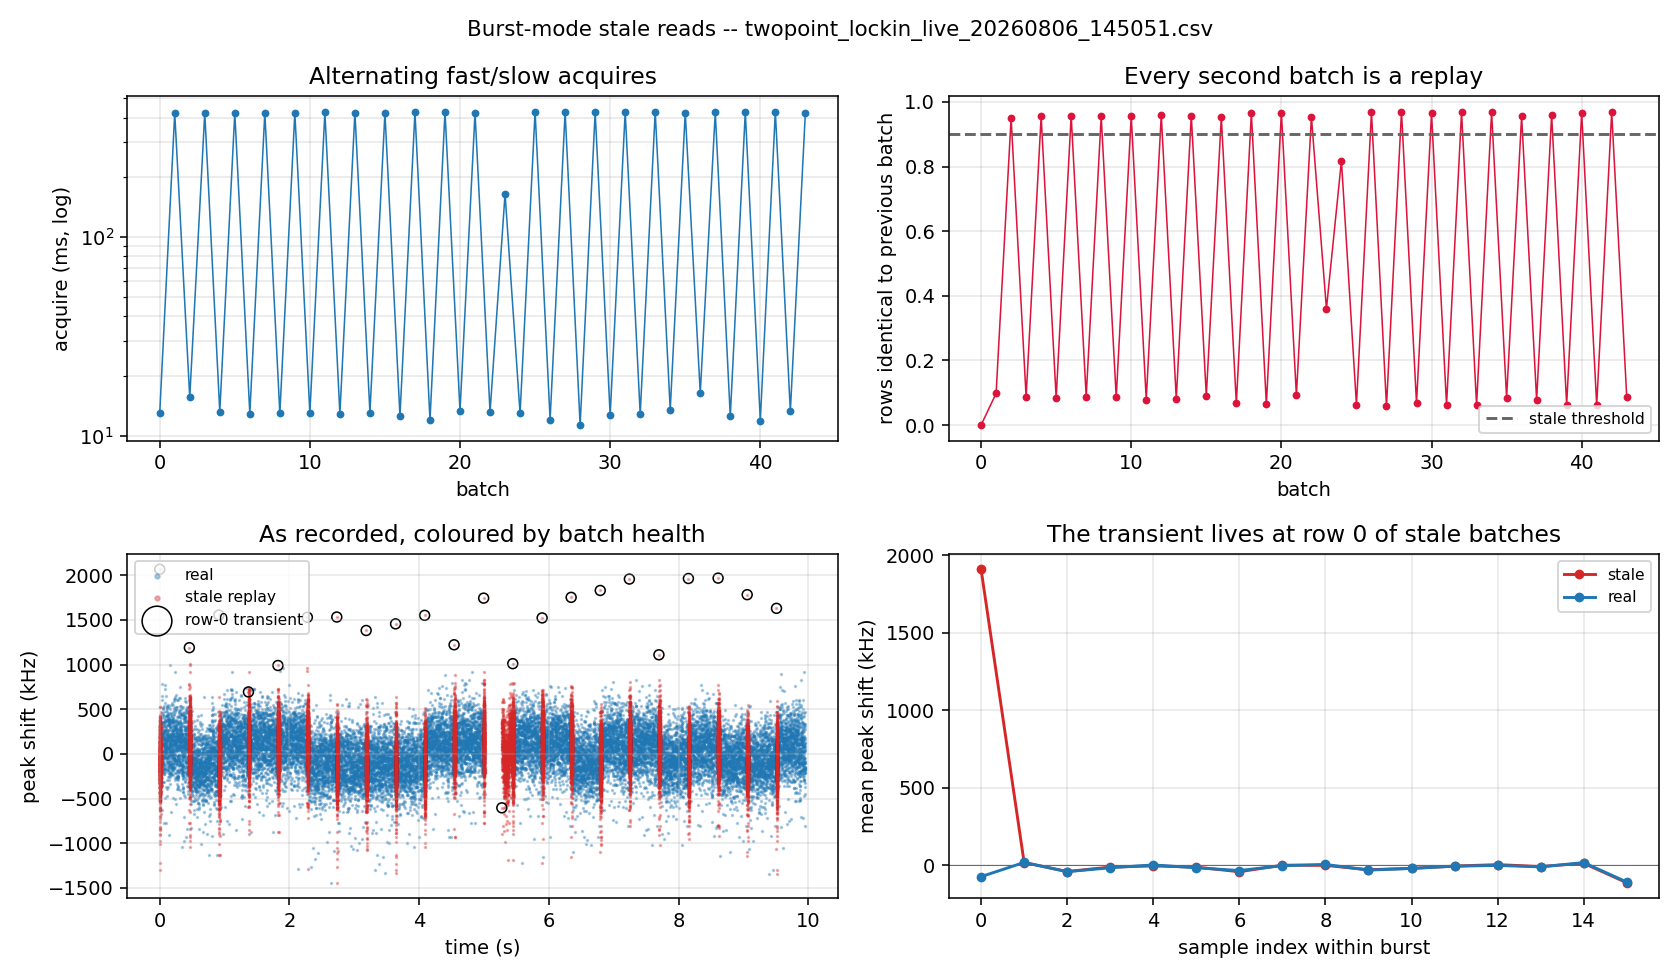
\includegraphics[width=\linewidth]{figures/burst_staleness.png}
\caption{Burst-mode stale reads on 2026-08-06. The stale replays (red) compress
into narrow vertical stripes because their 1000 samples are stamped across a 13\,ms
window while the real samples (blue) spread over 425\,ms. Circled points are the
row-0 transients --- one every $\sim$0.45\,s, exactly the periodicity seen in the
original plot.}
\end{figure}

\section{What to set}

\begin{center}
\small
\begin{tabular}{@{}llp{7.2cm}@{}}
\toprule
\hd{Parameter} & \hd{Recommended} & \hd{Why} \\
\midrule
\co{BURST_ON_STALE} & \co{"drop"} & Re-acquires, then \emph{skips} the batch rather
  than writing a replay to the CSV. Costs duty cycle, not correctness. \\
\co{BURST_STALE_RETRIES} & 2 & The race is transient; a repeat call usually lands
  on a completed run. \\
\co{BURST_REPS} & 500--1000 & See the rate table above; returns flatten past 1000
  and the time-series gaps grow. \\
\co{BURST_DROP_FIRST_REP} & \co{True} & Row 0 runs 1.4\% high --- a real transient. \\
\co{BURST_RESET_TPROC} & \co{True} & Kept available and harmless, but
  \textbf{measured not to fix the replay} (\S\ref{sec:replay}). \\
\bottomrule
\end{tabular}
\end{center}

\section{When to use it}

\textbf{Today, for best sensitivity: this is the mode.} 38\,\etaunit\ at an
effective 3.1\,kHz beats streaming by $\sim$6$\times$ and averaged mode by
7--13$\times$. The price is a 26\% duty cycle loss and a $\sim$15\,ms hole in the
time series every 135\,ms, which matters for a continuous MCG trace and does not
matter for a noise-floor measurement.

If the replay defect is ever fixed, this mode gets $\sim$15\% faster for free. If
the streaming noise defect is fixed, Method C becomes strictly better for
continuous recording.

\chapter{Method C --- Streaming mode}
\label{sec:stream}

\begin{center}
\small
\begin{tabular}{@{}ll@{}}
\toprule
Notebook cell & Step 4C (analysis: Step 5C) \\
Code path & \co{prog.stream(total_reps=N)} --- a generator \\
One packet returns & 38--500 reps, continuously, as they arrive \\
Measured rate & \textbf{1041.7\,Hz} (or 4167\,Hz with no host binning) \\
Rate limited by & the FPGA cadence alone \\
Duty cycle & \textbf{100.0\%} \\
Measured floor & 240\,\etaunit \\
Open defects & \Open{} \textbf{floor is $\sim$6$\times$ burst} (\S\ref{sec:streamnoise});
              25\% PL droop (\S\ref{sec:droop}) \\
\bottomrule
\end{tabular}
\end{center}

\section{Mechanics}

One \co{config_all}, one \co{start_readout(total_reps)}, then nothing but draining
the streamer queue with \co{poll_data()} in a loop. The board-side worker thread
transfers completed shots out of the accumulated buffer autonomously while the
tProc keeps running.

Because nothing is re-armed mid-run:

\begin{itemize}
  \item the replay race of Method B \textbf{cannot occur} --- there is no second
        configuration to race against;
  \item there is \textbf{no inter-burst gap} --- the FPGA never stops;
  \item timestamps follow the FPGA cadence \textbf{exactly}, rather than being
        reconstructed from host arrival times, which only record when the host
        happened to drain the queue.
\end{itemize}

\paragraph{\co{cfg.reps} is the run length.} The tProc loops \co{reps} times and
ends, so the rep count must be set before compilation and cannot change mid-run.
\co{stream()} raises if \co{cfg.reps != total_reps} rather than silently
truncating.

\paragraph{Host-side binning.} \co{STREAM_TARGET_HZ} sets an integer number of
reps to average on the host per output sample. Whole reps only, so the achieved
rate is the cadence divided by an integer rather than exactly the target: at
$\tau=\SI{120}{\micro\second}$, a 1000\,Hz target gives $\text{bin}=4$ and
therefore 1041.7\,Hz. Leftover reps carry into the next packet, so no rep is
dropped and no bin straddles a packet boundary.

\section{Timing budget, component by component}
\label{sec:streambudget}

\subsection*{Operating point: $\tau=\SI{120}{\micro\second}$, bin = 4 (2026-08-14)}

\begin{center}
\small
\begin{tabular}{@{}>{\raggedright\arraybackslash}p{4.3cm}rr>{\raggedright\arraybackslash}p{5.4cm}@{}}
\toprule
\hd{Component} & \hd{Per output sample} & \hd{Share} & \hd{How obtained} \\
\midrule
ADC integration ($4\times\SI{240}{\micro\second}$)
  & \textbf{\SI{960.0}{\micro\second}} & \textbf{100.0\%} & exact, Eq.~\ref{eq:recover}, $D$=147456 \\
Host RPC chain
  & \SI{0}{\micro\second} & 0\% & \textbf{paid once for the whole run} \\
Inter-packet gap
  & \SI{0}{\micro\second} & 0\% & the FPGA does not stop between packets \\
Timestamp jitter
  & \SI{0.0}{\micro\second} & 0\% & cadence-derived; min = max = \SI{960.0}{\micro\second} \\
\midrule
\textbf{TOTAL per output sample} & \textbf{\SI{960.0}{\micro\second}} & 100\% & measured spacing \\
Rate & \textbf{1041.67\,Hz} & & predicted 1041.67\,Hz --- \emph{exact} \\
Duty cycle & \textbf{100.0\%} & & 125\,000 reps $\times$ \SI{240}{\micro\second} in \SI{29.999}{\second} \\
\bottomrule
\end{tabular}
\end{center}

\begin{keybox}[This is what a clean timing budget looks like]
Every microsecond of the \SI{960}{\micro\second} sample period is ADC integration.
The measured sample spacing has \textbf{min = max = \SI{960.0}{\micro\second}} ---
zero jitter, because the timestamps come from the cadence rather than from arrival
times. Predicted and measured rate agree to the digit.

Compare Method A, where 79\% of the period is host overhead, and Method B, where
26\% is overhead and waste.
\end{keybox}

\section{Every parameter of the streaming cell, one at a time}
\label{sec:streamparams}

Step 4C has six knobs and three of them behave in ways that are not obvious from
their names. This section is the reference for all of them.

\subsection{\texorpdfstring{\co{STREAM_TARGET_HZ} and the bin}{STREAM\_TARGET\_HZ and the bin}}
\label{sec:bin}

You ask for a rate; the cell converts it into an integer number of reps to average
per output sample, and that integer --- not your request --- sets the rate:

\begin{equation}
\co{bin} = \max\!\left(1,\ \operatorname{round}\!\left(\frac{1}{\co{STREAM_TARGET_HZ}\times t_\text{rep}}\right)\right),
\qquad
f_\text{achieved} = \frac{1}{\co{bin}\times t_\text{rep}}.
\label{eq:bin}
\end{equation}

At $t_\text{rep}=\SI{240}{\micro\second}$, asking for \SI{1000}{\hertz} gives
$\co{bin}=\operatorname{round}(4.167)=4$ and therefore
\textbf{\SI{1041.7}{\hertz}}, not \SI{1000}{\hertz}. That is why every streamed
file in this project reports \SI{1041.7}{\hertz}: it is the nearest achievable
rate, and reps cannot be split.

Four things follow from the bin being a \emph{mean} of consecutive reps rather
than a decimation, and all four matter:

\begin{enumerate}
  \item \textbf{It averages, so it buys $\sqrt{\co{bin}}$ in $\sigma$.} Dropping
  3 of every 4 reps would not. At \co{bin} = 4 that is a factor of 2 --- the same
  free averaging Method A gets from filling the call floor (\S\ref{sec:freeavg}),
  obtained here without giving up any rate you were going to use.
  \item \textbf{It anti-aliases, at $1/(2\,\co{bin}\,t_\text{rep})$.} A boxcar of
  \co{bin} reps has its first null at $f_\text{achieved}$ and rolls off as
  $|\operatorname{sinc}|$ before it, so noise between $f_\text{achieved}/2$ and
  the raw \SI{4167}{\hertz} is suppressed rather than folded back in. This is the
  reason to bin in the acquisition cell rather than to record raw and decimate
  afterwards.
  \item \textbf{Bins never straddle a packet boundary.} Reps left over at the end
  of a packet are carried into the next one (\co{_pending} in the cell), so a bin
  is always \co{bin} consecutive reps of the same continuous run. Packet
  boundaries are an artefact of when the host drained the queue and mean nothing
  physical; a bin that straddled one would still be correct, but the carry makes
  the sample count exactly $\lfloor N_\text{reps}/\co{bin}\rfloor$ regardless of
  how the packets happened to land.
  \item \textbf{The timestamp is the bin centre.} \co{(first_rep + (i + 0.5) *
  bin) * cadence}. Using the bin's first rep would bias every sample early by
  $\co{bin}\,t_\text{rep}/2$ --- \SI{480}{\micro\second} at \co{bin} = 4.
\end{enumerate}

\begin{center}
\small
\begin{tabular}{@{}rrrl@{}}
\toprule
\hd{\co{bin}} & \hd{Per output sample} & \hd{Rate} & \hd{Note} \\
\midrule
1 & \SI{240}{\micro\second} & \textbf{4166.7\,Hz} & \co{STREAM_TARGET_HZ = None}; every rep kept \\
2 & \SI{480}{\micro\second} & 2083.3\,Hz & \\
\textbf{4} & \textbf{\SI{960}{\micro\second}} & \textbf{1041.7\,Hz} & what ran on 2026-08-14 and 2026-08-17 \\
8 & \SI{1920}{\micro\second} & 520.8\,Hz & \\
42 & \SI{10.08}{\milli\second} & 99.2\,Hz & equivalent averaging to Method A, at 100\% duty \\
\bottomrule
\end{tabular}
\end{center}

The last row is worth noting: streaming with \co{bin = 42} produces the same
averaging as the recommended Method A operating point, at the same rate, but with
100\% duty cycle instead of 21\% --- i.e. \emph{if the streaming noise excess were
resolved}, streaming would dominate Method A at every rate.

\subsection{\texorpdfstring{\co{STREAM_DURATION_SEC}, \co{total_reps} and \co{cfg.reps} --- all the same number}{STREAM\_DURATION\_SEC, total\_reps and cfg.reps}}

The tProc loops \co{cfg.reps} times and then ends. The rep count \emph{is} the
run length, it is compiled into the program, and it cannot be changed once the
program is uploaded. So the cell computes

\[
\co{total_reps} = \operatorname{round}\!\left(\frac{\co{STREAM_DURATION_SEC}}{t_\text{rep}}\right)
\]

\noindent and builds the program with \co{cfg.reps} set to it.
\co{stream()} raises \co{ValueError} if the two disagree rather than quietly
streaming a different length than you asked for. At \SI{30}{\second} and
$t_\text{rep}=\SI{240}{\micro\second}$ that is \num{125000} reps, giving
$\num{125000}/4 = \num{31250}$ samples --- which is exactly the row count of
every streamed CSV in the 2026-08-17 session.

There is no way to stop early and keep a valid file beyond interrupting the cell:
Ctrl-C ends the generator, the \co{finally} leaves the board idle, and
\co{stream_qc()["aborted"]} records that the run was short.

\subsection{\texorpdfstring{\co{poll_timeout_s} --- and why it is currently unreachable}{poll\_timeout\_s}}

\co{stream(poll_timeout_s=10.0)} is a client-side guard: if the board sends
nothing for this long, raise instead of waiting forever. It only does anything
when the poll is bounded, and as of the 2026-08-17 fix the poll is blocking by
default (\co{POLL_TIMEOUT_S = None}), so on the healthy path this guard is never
reached. That is deliberate, and \S\ref{sec:wedge} is the argument for it. What
protects an interrupted run is the generator's \co{finally}, not this timeout.

To arm it for a diagnostic run, set the class attribute for the session:

\begin{center}\co{MultipointLockinODMR.POLL_TIMEOUT_S = 5.0}\end{center}

\subsection{Stride, packet size and \texorpdfstring{\co{avg_maxlen}}{avg\_maxlen}}
\label{sec:stride}

None of these are host-side settings; they are consequences of the firmware and
the board worker, and they are what \co{stream_headroom()} reports.

\begin{center}
\small
\begin{tabular}{@{}l>{\raggedright\arraybackslash}p{10.4cm}@{}}
\toprule
\hd{Quantity} & \hd{What it is} \\
\midrule
\co{avg_maxlen} & Length of the accumulated buffer, in entries, from the
  firmware. One entry per readout per rep. \\
\co{reads_per_shot} & $n_\text{slots}\times n_\text{readouts per slot}$ --- 2 for
  the two-point default, \textbf{32} for a 16-point run with references. \\
\co{shots_that_fit} & \co{avg_maxlen // reads_per_shot}. The buffer budget is
  shared across every readout in a shot, so a 16-point run has sixteen times less
  room than a two-point one. \\
stride & \co{max(1, int(0.1 * shots_that_fit))}. The board worker transfers this
  many shots at a time --- 10\% of the buffer, chosen by qick, not by us. \\
packet size & Whatever the worker had ready when the host polled: on 2026-08-14,
  38--500 reps, median 205. It varies, and \emph{it does not matter}: the rep axis
  is carried in \co{first_rep}/\co{n_reps}, so the timestamps are exact regardless
  of how the data was parcelled up. \co{stream_qc()} proves that on the data. \\
\bottomrule
\end{tabular}
\end{center}

The failure mode is overflow: if unread samples ever reach \co{avg_maxlen}, the
worker raises and the run dies. Run \co{stream_headroom()} before a long stream
and check that \co{shots_that_fit} is several strides' worth. This has never bound
on the two-point path and is a live constraint on the multipoint one
(Ch.~\ref{ch:mpstream}).

\begin{openbox}[\co{stream_headroom()} silently failed for the whole 2026-08-17 session]
It read \co{qd.soc['readouts'][ch]['avg_maxlen']}, and \co{qd.soc} is a Pyro
\co{Proxy}: a proxy forwards \emph{method calls} but not \co{__getitem__}, so
this raised \co{'Proxy' object is not subscriptable} and the cell printed
``could not read avg_maxlen'' instead of a number. The subscriptable object is
\co{qd.soccfg}, the local \co{QickConfig} that qick's \co{make_proxy()} builds
from \co{soc.get_cfg()}. Fixed 2026-08-17; the check now runs.
\end{openbox}

\section{Verification: the guarantees, checked on the data}

Streaming's value is its exactness, so Step 5C checks it rather than assuming it.
On the 2026-08-14 run:

\begin{center}
\small
\begin{tabular}{@{}lrl@{}}
\toprule
\hd{Check} & \hd{Result} & \hd{Meaning} \\
\midrule
\co{rep_index} gaps & \textbf{0} & no reps dropped; cadence timestamps valid throughout \\
\co{rep_index} step & 4, uniformly & host binning consistent, no straddled bins \\
Duplicate rows & \textbf{0} of 31\,250 & the replay race really is absent \\
Reps collected & 125\,000 / 125\,000 & nothing lost \\
Packets & 152 & 38--500 reps each, median 205 \\
Duty cycle & 100.0\% & the FPGA never idled \\
\bottomrule
\end{tabular}
\end{center}

\co{stream()} also now refuses to reshape a packet whose payload size does not
match its own rep count. Such a packet would silently misalign every subsequent
sample and mix the two parked frequencies together --- which would look exactly
like a flat broadband noise excess. No occurrence has been observed, but it would
previously have been invisible.

\section{The buffer-overflow constraint}

The board worker transfers in strides of roughly 10\% of the accumulated buffer and
raises if unread samples reach \co{avg_maxlen}. \co{stream_headroom()} reports the
actual margin at runtime rather than assuming it:

\begin{center}
\co{\{avg_maxlen, reads_per_shot, shots_that_fit, seconds_that_fit, worker_stride_shots\}}
\end{center}

At $\tau=\SI{120}{\micro\second}$ with one read per shot the cadence is
$\sim$4\,kHz, so even a modest buffer allows a poll interval of order a second.
No overflow has been observed, and the 500-sample first packet is no noisier than
the 205-sample ones, which argues against overflow being behind the noise excess.

\section{The PL droop}
\label{sec:droop}

\begin{openbox}[Real, and specific to this mode]
With no gap between acquires the sample heats. On the 2026-08-14 run the PL fell
\textbf{25\% over 30\,s}, smoothly, from 993 to 744 ADC counts.

It is mostly common-mode and largely cancels in $z_+-z_-$: it is 85\% of the
\emph{common-mode} variance but only \textbf{2.8\%} of the $\Delta f$ variance. But
it walks the operating point down the flank, so the slopes the conversion assumes
drift out of validity over the run.

Step 5C detrends it (rolling median, corner $\sim f_s/\text{window}$) and reports
the magnitude. The proper fix is a periodic re-zero during the run, which is not
implemented.
\end{openbox}

\section{When to use it}

For anything that needs a \emph{continuous} record above a few hundred Hz --- MCG,
drone transients --- streaming is the only method that provides it: no gaps, exact
timestamps, 100\% duty cycle. Its rate is proven.

Its noise floor is currently $\sim$6$\times$ worse than burst, which for absolute
sensitivity work makes burst the better choice today. \textbf{Resolving
\S\ref{sec:streamnoise} is the single highest-value open item in this document},
because it would make streaming better than both other methods at every operating
point.

\chapter{Timing, in full}
\label{ch:timing}

Chapters~\ref{sec:avg}--\ref{sec:stream} gave each method's budget. This chapter
gives the evidence that the model behind them is right, and the practical
consequences.

\section{The evidence for a per-call floor}
\label{sec:floorevidence}

Applying the exact-recovery technique of \S\ref{sec:quantum} to all 21 usable
averaged runs across three sessions (\file{tables/timing.csv}):

\begin{center}
\small
\begin{tabular}{@{}llrrrr@{}}
\toprule
\hd{Session} & \hd{Config} & \hd{ADC integration} & \hd{Fastest call} & \hd{Median period} & \hd{Rate} \\
\midrule
2026-08-04 & $D$=654340  & \SI{4.26}{\milli\second} & 9.35--\SI{9.53}{\milli\second} & 10.48--\SI{10.62}{\milli\second} & 94--95\,Hz \\
2026-08-04 & $D$=706560  & \SI{4.60}{\milli\second} & \SI{9.29}{\milli\second} & \SI{10.84}{\milli\second} & 92\,Hz \\
2026-08-04/06 & $D$=1504982 & \SI{9.80}{\milli\second} & 9.61--\SI{10.29}{\milli\second} & 10.93--\SI{11.54}{\milli\second} & 87--91\,Hz \\
\textbf{2026-08-14} & $D$=368640 & \textbf{\SI{2.40}{\milli\second}} & 10.14--\SI{10.30}{\milli\second} & 11.26--\SI{11.52}{\milli\second} & 87--89\,Hz \\
\textbf{2026-08-14} & $D$=847872 & \textbf{\SI{5.52}{\milli\second}} & \SI{10.27}{\milli\second} & \SI{11.39}{\milli\second} & 87.8\,Hz \\
\bottomrule
\end{tabular}
\end{center}

Two runs were excluded from the fit below because their loop period exceeds
1.5$\times$ their acquire time --- most of it was spent outside \co{acquire()}
(live plotting on, or operator interaction), so they say nothing about the call.

\begin{figure}[H]
\centering
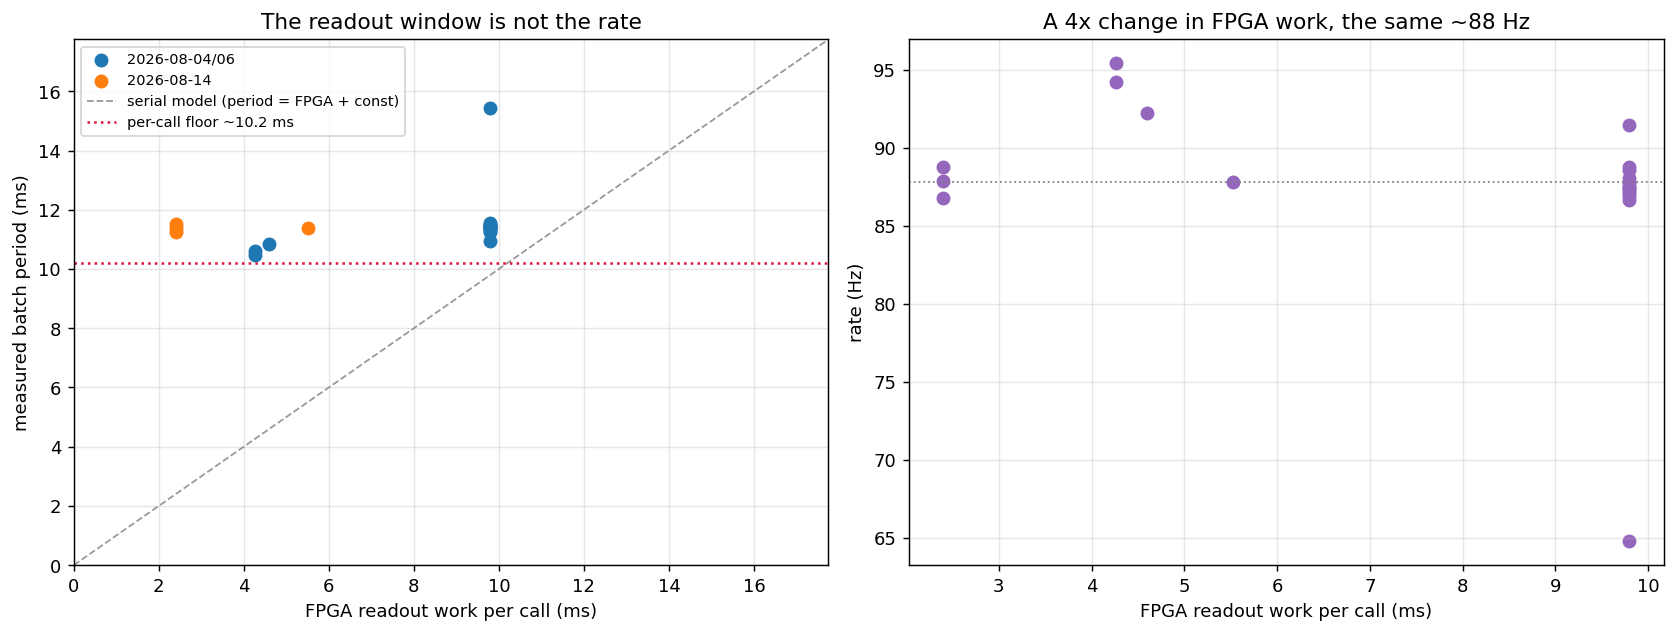
\includegraphics[width=\linewidth]{figures/timing_floor.png}
\caption{Left: measured batch period against FPGA readout work. The dashed line is
the serial model the data does not follow; the red dotted line is the per-call
floor. Right: the same data as rate --- a 4$\times$ change in FPGA work leaves the
rate at $\sim$88\,Hz.}
\end{figure}

\subsection{Argument 1 --- the slope is not 1}

Fitted \emph{within} a session, because comparing across sessions would confound
the FPGA change with the floor itself, which moved $\sim$1\,ms between 2026-08-04/06
and 2026-08-14:

\begin{center}
\small
\begin{tabular}{@{}lrrr@{}}
\toprule
\hd{Session} & \hd{FPGA work} & \hd{Period} & \hd{$d(\text{period})/d(\text{FPGA})$} \\
\midrule
2026-08-04/06 & 4.26 $\rightarrow$ \SI{9.80}{\milli\second} (2.3$\times$) & 10.55 $\rightarrow$ \SI{11.43}{\milli\second} & \textbf{+0.140} \\
2026-08-14    & 2.40 $\rightarrow$ \SI{5.52}{\milli\second} (2.3$\times$) & 11.38 $\rightarrow$ \SI{11.39}{\milli\second} & \textbf{+0.003} \\
\bottomrule
\end{tabular}
\end{center}

A serial model $\text{period} = \text{host} + \text{FPGA}$ requires slope
$= 1.000$. Neither session comes close.

\subsection{Argument 2 --- no serial model fits at all}

The 2026-08-14 runs used \SI{2.40}{\milli\second} of FPGA work, and their
\emph{fastest} call was \SI{10.14}{\milli\second}. Under a serial model that
demands a host term of \SI{7.74}{\milli\second}, against the
\SI{1.60}{\milli\second} the 2026-08-06 analysis reported for the same code on the
same rig eight days earlier. There is no constant, non-negative host term that
fits both sessions.

Under the max-model both are consistent: the host chain is $\sim$10--11.4\,ms in
both, and the FPGA work is simply hidden inside it.

\subsection{Argument 3 --- the wobble is entirely in the call}

The instantaneous rate spans 81.4--100.1\,Hz, which is what is seen live as
``85--97\,Hz''. Decomposing it:

\begin{itemize}
  \item The FPGA term is \textbf{deterministic} --- 23 reps of identical pulse work
        vary by well under a microsecond, and the burst runs confirm the cadence is
        stable to 0.4\% across runs.
  \item \co{acq_seconds} spans 10.1--\SI{12.1}{\milli\second} (jitter
        1.6--\SI{1.9}{\milli\second} p95$-$p05).
  \item Python outside the call stays at \SI{0.06}{\milli\second}.
\end{itemize}
So \textbf{100\% of the wobble is host/network scheduling inside \co{acquire()}} ---
Windows scheduling plus TCP/Pyro latency on stages 1--6.

\section{The corrected model}
\label{sec:model}

\begin{equation}
\boxed{\;
\text{period} \;=\; \max\bigl(\underbrace{H}_{\text{host call}},\;
\underbrace{\text{reps}\times t_\text{rep}}_{\text{FPGA}}\bigr) \;+\; \underbrace{P}_{\text{Python, }\sim\SI{0.06}{\milli\second}}
\;}
\label{eq:model}
\end{equation}

with, on this rig,
\[
H_\text{typical} = \SI{11.4}{\milli\second}, \qquad
H_\text{floor} = \SI{10.1}{\milli\second}.
\]

Two constants rather than one, because the two uses want different ends of the
distribution: $H_\text{typical}$ predicts the rate, $H_\text{floor}$ sizes the free
averaging (fill past the fastest call and even the quick calls become FPGA-bound).

\subsection{Predicted against measured}

\begin{center}
\small
\begin{tabular}{@{}llrrrr@{}}
\toprule
\hd{$\tau$} & \hd{reps} & \hd{FPGA} & \hd{Old model} & \hd{Eq.~\ref{eq:model}} & \hd{Measured} \\
\midrule
\SI{213}{\micro\second} & 23 & \SI{9.80}{\milli\second} & 160\,Hz & \textbf{87.7\,Hz} & 87.5\,Hz \\
\SI{120}{\micro\second} & 23 & \SI{5.52}{\milli\second} & 400\,Hz & \textbf{87.7\,Hz} & 87.8\,Hz \\
\SI{120}{\micro\second} & 10 & \SI{2.40}{\milli\second} & 180\,Hz & \textbf{87.7\,Hz} & 86.8\,Hz \\
\bottomrule
\end{tabular}
\end{center}

The model giving the \emph{same} answer for all three is the point.

\co{measure_host_floor()} calibrates $H$ on the rig in about a second, using a
\co{reps=1} probe whose FPGA work is \SI{240}{\micro\second} --- so whatever the
call still costs is the host chain, measured rather than inferred. Step 4A calls it
at startup. Given that $H$ already differs by \SI{1.2}{\milli\second} between the
two sessions, the defaults above should be treated as a starting point.

\section{Free averaging}
\label{sec:freeavg}

\begin{keybox}[The most actionable consequence in this document]
If the FPGA work hides under the call, then \textbf{running fewer reps than fit is
pure loss}. The call takes the same wall-clock time either way, so the unused
milliseconds are photons that were never collected.
\end{keybox}

At $\tau=\SI{120}{\micro\second}$, $t_\text{rep}=\SI{240}{\micro\second}$, so
$H_\text{floor}/t_\text{rep} = 10.1/0.240 = \textbf{42 reps}$ fit inside the floor.
The 2026-08-14 runs used \textbf{10}.

\begin{center}
\small
\begin{tabular}{@{}rrrrl@{}}
\toprule
\hd{reps} & \hd{FPGA} & \hd{Duty cycle} & \hd{Rate} & \hd{Note} \\
\midrule
10 & \SI{2.40}{\milli\second} & 21\% & 87.7\,Hz & what ran \\
23 & \SI{5.52}{\milli\second} & 48\% & 87.7\,Hz & \\
\textbf{42} & \textbf{\SI{10.08}{\milli\second}} & \textbf{88\%} & \textbf{87.7\,Hz} & the fill point \\
50 & \SI{12.00}{\milli\second} & 100\% & 83.3\,Hz & now FPGA-bound; rate starts to fall \\
100 & \SI{24.00}{\milli\second} & 100\% & 41.7\,Hz & \\
\bottomrule
\end{tabular}
\end{center}

Implemented as \co{reps_that_fit()}, used automatically when
\co{AVG_REPS_PER_BATCH = None}. \co{describe_timing()} prints the headroom:

\begin{quote}\small\ttfamily
2 freqs, order=forward (2 slots/rep), tau=120.0 us, 10 reps -> 240 us/rep, 2.40 ms FPGA work\\
\ \ averaged mode: 2.40 ms of FPGA work hides under the 10.1 ms per-call floor (24\% used) -> 87.7 Hz\\
\ \ FREE AVERAGING: 42 reps also fit inside the floor. Raising 10 -> 42 costs no rate\\
\ \ \ \ \ \ \ \ \ \ \ \ \ \ \ \ and buys up to 2.0x in sigma if the noise is white.
\end{quote}

\begin{openbox}[The caveat is in that last clause]
``\emph{if the noise is white}'' --- and \S\ref{sec:notshot} shows it currently is
not. The averaged mode's noise does not average down at all; it gets \emph{worse}
with more reps. Filling the budget is still free, so it is still worth doing, but
do not expect the full $\sqrt{4.2}=2.0\times$ until the per-acquire noise term is
understood.
\end{openbox}

\section{Knob by knob}
\label{sec:knobs}

\begin{center}
\small
\begin{tabular}{@{}lp{3.6cm}p{4.0cm}p{3.4cm}@{}}
\toprule
\hd{Knob} & \hd{Effect on rate} & \hd{Effect on sensitivity} & \hd{Verdict} \\
\midrule
\co{readout_integration_tus} ($\tau$) &
  \textbf{None} in averaged mode below the floor; \emph{is} the cadence in burst/stream &
  Flat for $\tau\le\SI{140}{\micro\second}$, worse above (\S\ref{sec:window}) &
  Not a rate lever in Method A. Keep at \SI{120}{\micro\second} \\[3pt]
\co{reps} &
  \textbf{None} below the floor; linear above &
  Should be $1/\sqrt{N}$; measured far less (\S\ref{sec:notshot}) &
  Free averaging up to the floor \\[3pt]
Acquisition method &
  \textbf{12--47$\times$} &
  See Chapter~\ref{ch:sensitivity} &
  \textbf{The only real rate lever} \\[3pt]
\co{multipoint_skip_reference} &
  2$\times$ (already on) &
  Removes a contaminated normaliser &
  Keep on \\[3pt]
\co{multipoint_pair_order} &
  2$\times$ per rep for \co{"abba"} &
  Cancels linear common-mode drift; free at equal averaging &
  \Open{}, untested \\[3pt]
\co{n_freqs} & Linear & 2 is the minimum for a two-point estimator & Fixed at 2 \\[3pt]
\co{BURST_REPS} & Sub-linear; flattens past $\sim$1000 & None directly & 500--1000 \\[3pt]
\co{STREAM_TARGET_HZ} & Sets the bin divisor exactly & $1/\sqrt{\text{bin}}$ if white & Free choice \\[3pt]
\co{LIVE_SHOW_PLOT} & 20--100\,ms per redraw & None & Keep \co{False} \\[3pt]
\co{SAVE_EVERY_SEC} rewrite & 25--220\,ms every 5\,s & None & Fixed: append-only \\
\bottomrule
\end{tabular}
\end{center}

\section{The 1\,kHz question, closed}

The 2026-08-06 analysis concluded that 1\,kHz was unreachable with one call per
sample. That conclusion \textbf{survives the retraction and in fact gets stronger}:
the per-call cost is $\sim$11\,ms, not 1.6\,ms, so a 1\,ms period is unreachable by
a factor of eleven rather than by 1.6.

The route it identified --- one \co{start_readout} with continuous polling --- was
built, and on 2026-08-14 it delivered \textbf{1041.7\,Hz} exactly as designed
(\S\ref{sec:streambudget}). The rate target is met. Only its noise is open.

\chapter{Sensitivity and noise}
\label{ch:sensitivity}

\section{The readout-window optimum}
\label{sec:window}

From 92 ODMR sweeps at 17 readout windows on 2026-08-06
(\file{docs/2026-08-06\_twopoint\_timing/tables/integration\_time.csv}). Lorentzian
fits over 2840--2900\,MHz; noise taken from the point-to-point scatter of the
off-resonance wings, which is immune to slow drift across the sweep.

\begin{center}
\small
\begin{tabular}{@{}rrrrrrr@{}}
\toprule
\hd{$\tau$ (\us)} & \hd{contrast} & \hd{$\sigma_z$} & \hd{$\sigma_z\sqrt{\tau}$} & \hd{$\sigma(\Delta f)$ kHz} & \hd{$t_\text{rep}$ \us} & \hd{$\eta$ \etaunit} \\
\midrule
50  & 0.541 & 3.01e-3 & 0.0213 & 51.3 & 109 & $186\pm14$ \\
90  & 0.517 & 2.13e-3 & 0.0202 & 37.0 & 189 & $\mathbf{177\pm14}$ \\
110 & 0.515 & 1.90e-3 & 0.0199 & 33.7 & 229 & $\mathbf{178\pm8}$ \\
\textbf{120} & 0.514 & 1.98e-3 & 0.0217 & 34.9 & 249 & $192\pm17$ \\
130 & 0.507 & 1.70e-3 & 0.0194 & 30.6 & 269 & $\mathbf{175\pm15}$ \\
140 & 0.506 & 1.71e-3 & 0.0202 & 30.6 & 289 & $181\pm7$ \\
170 & 0.513 & 2.01e-3 & 0.0262 & 35.6 & 349 & $232\pm5$ \\
190 & 0.495 & 2.09e-3 & 0.0288 & 38.4 & 389 & $264\pm22$ \\
\textbf{213} & 0.531 & 1.52e-3 & 0.0222 & 25.9 & 435 & $188\pm14$ \\
\bottomrule
\end{tabular}
\end{center}

Three results:

\begin{enumerate}
  \item \textbf{Contrast is flat} (0.49--0.54) across the whole range. A longer
        window buys no signal.
  \item \textbf{$\sigma_z\sqrt{\tau}$ is flat below $\sim$\SI{140}{\micro\second}
        (0.0207) and rises above it (0.0252).} Below \SI{140}{\micro\second} the
        readout averages down as $\sqrt{\text{time}}$; above it, the extra window
        length collects drift instead of statistics. \emph{This is the physical
        reason an optimum exists.}
  \item \textbf{$\eta$ is flat at $185\pm7$\,\etaunit\ for
        $\tau\le\SI{140}{\micro\second}$}, degrading to $232\pm20$ over
        150--\SI{200}{\micro\second}. Individual windows inside the flat band are
        not distinguishable --- the sweep-to-sweep scatter at fixed $\tau$ is
        $\pm14$, larger than the spread between them.
\end{enumerate}

\begin{figure}[H]
\centering
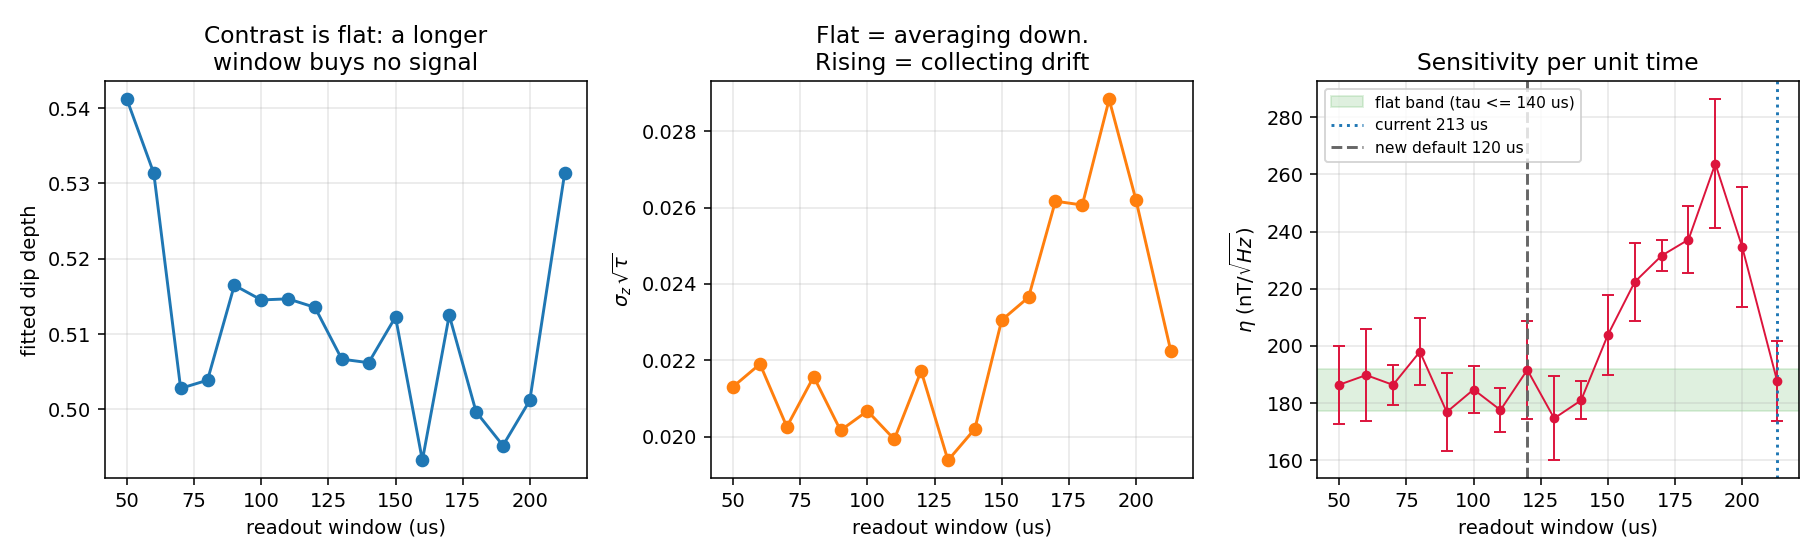
\includegraphics[width=\linewidth]{figures/integration_time.png}
\caption{Contrast, noise scaling and sensitivity against readout window, 2026-08-06.}
\end{figure}

\paragraph{Decision: $\tau = \SI{120}{\micro\second}$.} Inside the flat band, and
1.75$\times$ faster \emph{per rep} than \SI{213}{\micro\second}. Note carefully
that this does \textbf{not} make Method A faster (Chapter~\ref{ch:timing}) --- it
makes burst and streaming faster, and it lets more reps fit under Method A's call
floor.

\begin{openbox}[Two caveats that remain]
\textbf{The \SI{213}{\micro\second} point is an outlier.} It reads
188\,\etaunit, well below the 150--\SI{200}{\micro\second} trend it should
continue, on an unusually low $\sigma_z$ (1.52e-3). It was the configured default,
so those sweeps were probably taken under different conditions. The
$\sigma_z\sqrt{\tau}$ trend across 150--\SI{200}{\micro\second} is the more
reliable signal.

\textbf{The shape assumes \co{reps} was constant across the scan.} That is the
natural reading of a one-variable scan, and it is what flat $\sigma_z\sqrt{\tau}$
implies, but \co{reps} is not recorded in the sweep CSVs and cannot be recovered
from file timestamps (those gaps are dominated by operator cadence: median 4\,s
while $t_\text{rep}$ varies 4$\times$). A reps change part-way through could mimic
the rise above \SI{140}{\micro\second}.
\end{openbox}

\section{Measured sensitivity, per method}
\label{sec:etameas}

From \file{tables/modes.csv}. Both conventions of \S\ref{sec:conventions} are
given; when they disagree, trust the floor.

\begin{center}
\small
\begin{tabular}{@{}llrrrrr@{}}
\toprule
\hd{Session} & \hd{Method} & \hd{Run} & \hd{Rate} & \hd{$\sigma(\Delta f)$} & \hd{$\eta$} & \hd{Floor} \\
\midrule
08-14 & averaged & 144602 & 87.8\,Hz & 56.4\,kHz & 304 & 278 \\
08-14 & averaged & 144655 & 88.8\,Hz & 98.1\,kHz & 526 & 501 \\
08-14 & averaged & 145010 & 87.9\,Hz & 92.1\,kHz & 496 & 486 \\
08-14 & averaged & 145321 & 86.8\,Hz & 54.6\,kHz & 296 & 274 \\
08-14 & \textbf{stream} & 145442 & \textbf{1041.7\,Hz} & 160.8\,kHz & 251 & 240 \\
08-14 & \textbf{burst} & 150458 & 4166.7\,Hz (3089 net) & 71.4\,kHz & 56 & \textbf{38} \\
\midrule
08-06 & averaged & 144936 & 86.7\,Hz & 95.0\,kHz & 515 & 499 \\
08-06 & burst & 145051 & 2347\,Hz (2108 net) & 256.1\,kHz & 267 & 158 \\
\bottomrule
\end{tabular}
\end{center}
\emph{($\eta$ and floor in \etaunit.)}

\begin{figure}[H]
\centering
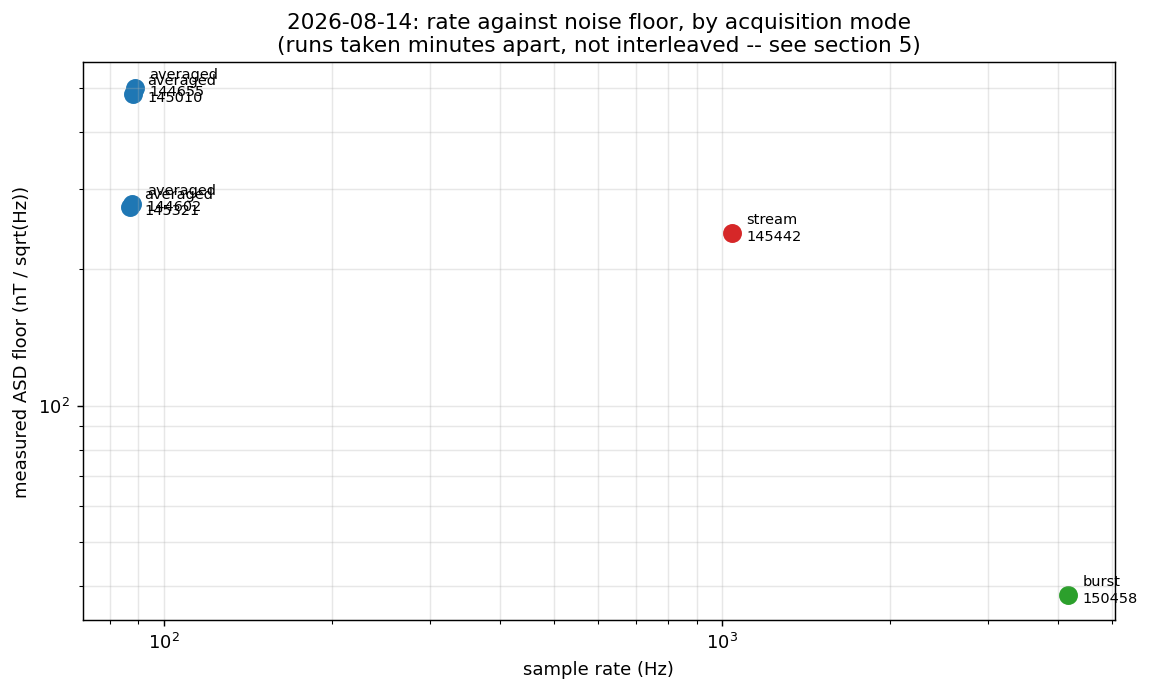
\includegraphics[width=0.86\linewidth]{figures/mode_comparison.png}
\caption{Rate against measured noise floor by method, 2026-08-14. The runs were
taken minutes apart rather than interleaved --- see the warning below.}
\end{figure}

\subsection{The photodiode fix: 4.1\texorpdfstring{$\times$}{x}}

\begin{keybox}[The headline sensitivity result]
Burst-mode noise floor, same two parked points, same measurement:
\[
\text{2026-08-06: } 158\,\text{\etaunit}
\quad\longrightarrow\quad
\text{2026-08-14: } \mathbf{38}\,\text{\etaunit}
\qquad (\mathbf{4.1\times})
\]
attributable to the reference-photodiode gain correction and the removal of signal-diode
saturation. Burst mode is the only method that currently shows the full benefit.
\end{keybox}

\subsection{A warning about comparing these rows}

\begin{openbox}[These runs are not strictly comparable]
They were taken minutes apart, not interleaved, and \S\ref{sec:notshot} shows the
per-rep noise varied \textbf{3.6$\times$} between two averaged runs \textbf{three
minutes apart} with identical settings (145010 vs 145321: 5.97\% vs 2.45\%).

Any A/B comparison across separate runs on this rig is unreliable. Only interleaved
measurements settle a method comparison, which is why the rig test in
\S\ref{sec:rigchecks} interleaves. Treat the method ranking above as indicative.
\end{openbox}

\section{Averaging does not buy \texorpdfstring{$\sqrt{N}$}{sqrt(N)}}

Block-averaging the real burst samples within each burst, 2026-08-06:

\begin{center}
\small
\begin{tabular}{@{}rrrr@{}}
\toprule
\hd{reps averaged} & \hd{$\sigma(\Delta f)$ kHz} & \hd{ideal $1/\sqrt{N}$} & \hd{excess} \\
\midrule
1   & 248.6 & 248.6 & 1.00 \\
4   & 141.0 & 124.3 & 1.13 \\
8   & 110.8 & 87.9  & 1.26 \\
\textbf{23}  & \textbf{86.7} & \textbf{51.8} & \textbf{1.67} \\
64  & 76.5  & 31.1  & 2.46 \\
128 & 72.3  & 22.0  & 3.29 \\
\bottomrule
\end{tabular}
\end{center}

The predicted 86.7\,kHz at $N=23$ matches the averaged runs, which came in at
73--110\,kHz for 11 of 12 runs (median 94\,kHz) --- an independent consistency
check, since the two are measured in completely different modes. But the excess
grows with $N$: past $\sim$30 reps, averaging is nearly free of benefit.

\begin{figure}[H]
\centering
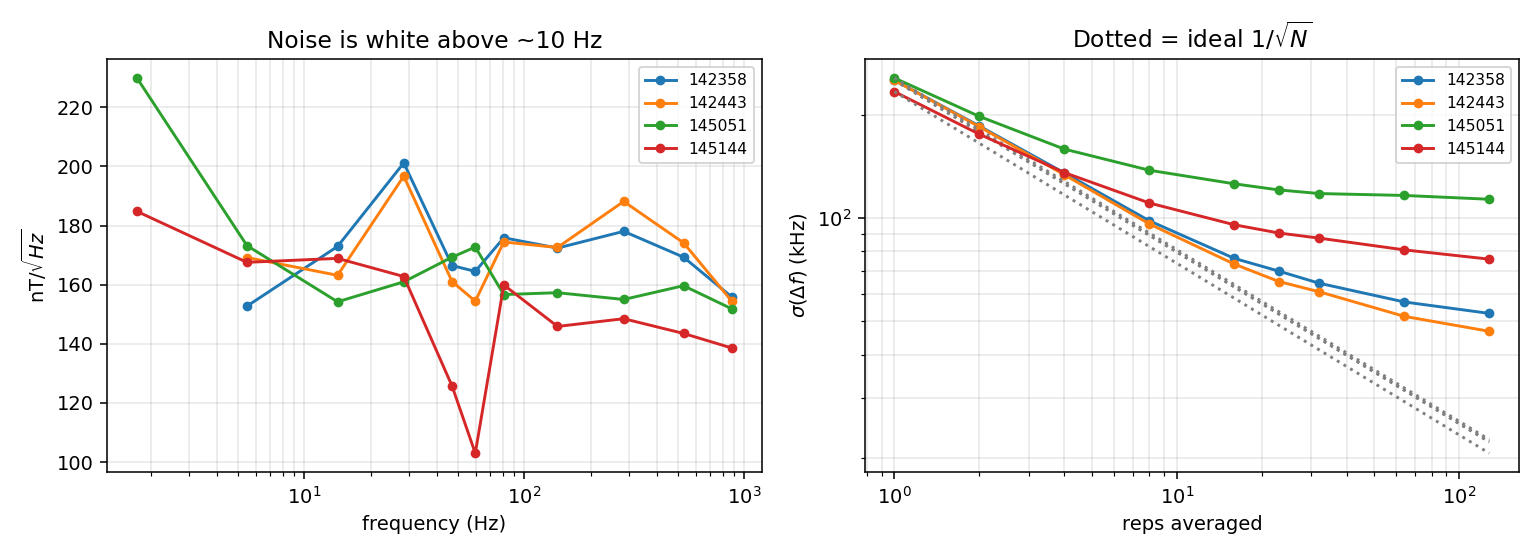
\includegraphics[width=\linewidth]{figures/noise_structure.png}
\caption{Noise spectrum and block-averaging behaviour, 2026-08-06. Above
$\sim$10\,Hz the spectrum is white at $\sim$165\,\etaunit; the excess is all below
10\,Hz.}
\end{figure}

\section{The noise is not photon shot noise}
\label{sec:notshot}

This is the sharpest version of the same finding, and the most important open item
in the document. Per-rep normalised-PL noise, scaled back from whatever averaging
each run used (\file{tables/per_rep_noise.csv}):

\begin{center}
\small
\begin{tabular}{@{}llrrr@{}}
\toprule
\hd{Session} & \hd{Method} & \hd{reps averaged} & \hd{per-rep $\sigma(z)$} & \hd{relative} \\
\midrule
2026-08-06 & burst    & 1  & 0.0076 & \textbf{0.67\%} \\
2026-08-06 & burst    & 1  & 0.0091 & \textbf{0.83\%} \\
2026-08-06 & averaged & 23 & 0.0114 & 1.11\% \\
2026-08-06 & averaged & 23 & 0.0161 & 1.38\% \\
\textbf{2026-08-14} & \textbf{burst} & 1 & \textbf{0.0059} & \textbf{0.61\%} \\
2026-08-14 & averaged & 10 & 0.0214 & 2.45\% \\
2026-08-14 & averaged & 10 & 0.0513 & 5.97\% \\
2026-08-14 & averaged & 23 & 0.0755 & \textbf{8.95\%} \\
2026-08-14 & stream   & 4  & 0.0522 & 7.57\% \\
\bottomrule
\end{tabular}
\end{center}

Two observations:

\begin{enumerate}
  \item \textbf{Burst is reproducibly 0.61--0.83\% in both sessions; everything
        else is 1.1--9\%.} Burst measures the per-rep noise \emph{directly}; the
        other rows infer it by scaling up a reps-averaged $\sigma$. The gap means
        the inference is wrong --- the noise in those modes is not a per-rep term.
  \item \textbf{Averaged mode gets \emph{worse} with more reps} (10 reps
        $\rightarrow$ 2.45\%, 23 reps $\rightarrow$ 8.95\%). Shot noise cannot do
        that.
\end{enumerate}

\begin{openbox}[OPEN --- the per-acquire noise term]
The dominant noise term is \textbf{per-acquire, not per-rep}, so it survives
averaging entirely. \textbf{If it were removed, Method A would inherit Method B's
4$\times$ better noise at no cost in rate}, and free averaging
(\S\ref{sec:freeavg}) would deliver its full $\sqrt{N}$.

Candidate mechanisms, none tested: a start-of-batch transient whose amplitude
varies with the (jittery) idle gap between calls; ADC offset drift re-sampled per
call; laser/MW state settling after the gap. The row-0 transient measured in burst
mode (+1.4\%) is direct evidence that \emph{something} happens at a batch boundary.

Protocol: \S\ref{sec:rigchecks}, check S6.
\end{openbox}

\section{Mains pickup and aliasing}
\label{sec:alias}

From \file{tables/spectra.csv}:

\begin{center}
\small
\begin{tabular}{@{}lrrrl@{}}
\toprule
\hd{Method} & \hd{Rate} & \hd{Strongest line} & \hd{Excess over floor} & \hd{60\,Hz appears at} \\
\midrule
averaged & 86.8--88.8\,Hz & --- & --- & \textbf{26.8--28.8\,Hz (aliased)} \\
stream   & 1041.7\,Hz & 61.7\,Hz & \textbf{10.2$\times$} & 60\,Hz \\
burst    & 4166.7\,Hz & 58.5\,Hz & 3.0$\times$ & 60\,Hz \\
\bottomrule
\end{tabular}
\end{center}

The mains line is real and strong --- \textbf{10$\times$ the noise floor} in the
streamed data, with odd harmonics at 185, 308 and 465\,Hz.

\begin{keybox}[At 88\,Hz, 60\,Hz folds to $\sim$27\,Hz and becomes unfixable]
Nyquist at 87.9\,Hz is 43.9\,Hz, so a 60\,Hz tone aliases to
$|60 - 87.9| = 27.9$\,Hz --- the middle of the measurement band. Once folded there
it is indistinguishable from a real 27.9\,Hz signal, and notching it would remove
real signal along with it.

This is a structural argument for running at $\ge$1\,kHz for drone and MCG work,
\emph{independent of sensitivity}: only there can the pickup be identified for what
it is and removed. \co{twopoint_spectra.alias_report()} raises this automatically
and Step 5A prints it on every averaged run.
\end{keybox}

Note that the 2026-08-06 analysis reported ``no 60\,Hz line''. That was correct for
what it could see: at 87.5\,Hz the line is not \emph{at} 60\,Hz, and the burst runs
of that session, which could have resolved it, were half replays with a badly
compressed time axis. The line was there all along.

\chapter{Open defects}
\label{ch:defects}

\section{Burst mode replays about half of every run}
\label{sec:replay}

\subsection{The evidence}

Every burst run in both sessions shows the same signature: acquires strictly
alternate short and long, and the short ones return a \emph{bit-identical} copy of
the previous batch.

\begin{center}
\small
\begin{tabular}{@{}lrrrrrr@{}}
\toprule
\hd{Run} & \hd{Batches} & \hd{Stale} & \hd{Fraction} & \hd{Pattern} & \hd{Recorded} & \hd{True} \\
\midrule
2026-08-06 \co{_142358} & 211 & 106 & 50.2\% & 13 / 425\,ms & 3911\,Hz & \textbf{1946\,Hz} \\
2026-08-06 \co{_142443} & 66  & 33  & 50.0\% & 13 / 424\,ms & 4182\,Hz & \textbf{2091\,Hz} \\
2026-08-06 \co{_145051} & 44  & 23  & 52.3\% & 13 / 425\,ms & 4421\,Hz & \textbf{2110\,Hz} \\
2026-08-06 \co{_145144} & 14  & 7   & 50.0\% & 13 / 425\,ms & 4455\,Hz & \textbf{2227\,Hz} \\
\textbf{2026-08-14 \co{_150458}} & \textbf{371} & \textbf{185} & \textbf{49.9\%} & 12 / 120\,ms & 6161\,Hz & \textbf{3089\,Hz} \\
\bottomrule
\end{tabular}
\end{center}

The separation is clean with nothing in between: the duplicate fraction is
\textbf{0.957 in the fast batches} and 0.069 in the real ones. Within a stale batch
the only rows that differ from the previous batch are row 0 and a block around rows
770--818 --- and 819 is exactly the streamer's transfer stride,
$0.1\times\co{avg_maxlen}/\co{reads_per_shot}$.

Detection uses two independent tests, either of which condemns a batch:
\begin{enumerate}
  \item $\ge$90\% of rows identical to the previous batch;
  \item wall-clock duration under half the FPGA work the batch claims to contain.
\end{enumerate}
Both are needed. On \co{_145051}, batch 24 is 82\% duplicate --- under the fraction
threshold, because the run's one CSV-flush stall shifted the alignment --- but
returned in \SI{12.9}{\milli\second} against \SI{425}{\milli\second} of claimed
pulse work.

\subsection{The 2026-08-06 root cause, and why it is now disproved}

\begin{retractbox}[DISPROVED --- \co{config_all} / \co{reset_tproc} was not the mechanism]
The 2026-08-06 analysis found a real bug. \co{qickdawg} called
\co{config_all(..., load_pulses=...)}, but \co{qick} 0.2.386 names that parameter
\co{load_envelopes}. \textbf{Every acquire raised \co{TypeError}}, was silently
caught, and fell back to \co{config_all(soc)} with \co{reset=False} --- and
\co{reset=False} means \co{stop_tproc(lazy=True)}, which \co{qick} documents as a
no-op on tProc v1. \textbf{The tProc was never stopped between runs}, so the
accumulated buffer was re-armed under a possibly-still-running program.

That was fixed on 2026-08-12 (commit \co{942d9e8}) and a \co{reset_tproc=}
argument was threaded through \co{acquire()}.

\textbf{The 2026-08-14 run used the fix and the replay fraction did not change}:
49.9\% (185/371). The rig was definitely running the new code --- $\tau$ =
\SI{120}{\micro\second} took effect and the new streaming cell produced output.

So the keyword bug was real and worth fixing, but it was \emph{not} the cause of
the replay. \textbf{The root cause is unknown.}
\end{retractbox}

What the elimination does tell us: the mechanism is not the tProc failing to stop,
because forcing the stop changes nothing. The remaining candidates involve the
accumulated buffer or the shot counter rather than the program:

\begin{itemize}
  \item \co{config_bufs()} re-arming the accumulator without clearing the counter,
        so \co{poll_data} returns the previous run's completed shots as if they were
        new;
  \item the board-side worker thread from the previous \co{start_readout} not being
        joined, so its queue still holds the old transfer;
  \item \co{start_readout}'s shot counter being read before the tProc has reset it.
\end{itemize}
None has been tested. A single instrumented burst run on the rig, printing the shot
counter and the queue depth before and after each \co{start_readout}, would
discriminate.

\subsection{Mitigation, which is in place}

\co{cfg.multipoint_on_stale = "drop"} makes the freshness guard re-acquire
(\co{multipoint_stale_retries}, default 2) and, if every attempt still returns the
same buffer, return \co{None} so the caller \textbf{skips the batch}. A replay is
never written to the CSV as though it were data.

This costs duty cycle, not correctness --- the recorded rate becomes honest:
3089\,Hz rather than the 6161\,Hz the raw file claims. Simulated against a board
that replays every second call, all 20 requested batches were recovered as real
data.

The guard is a byte comparison (\co{blake2b}) against the previous raw buffer, so it
costs microseconds and catches the failure \emph{whatever} its mechanism --- which
is why it survived the root cause being wrong.

\section{Streaming's noise floor is about 6\texorpdfstring{$\times$}{x} the burst floor}
\label{sec:streamnoise}

\subsection{The evidence}

Streaming and burst ran ten minutes apart at the same $\tau$, on the same hardware,
with nothing changed on the bench (confirmed with the operator). Their amplitude
spectral densities differ by a \textbf{flat factor of $\sim$6 across the whole
band} (\file{tables/read_path.csv}):

\begin{center}
\small
\begin{tabular}{@{}lrrr@{}}
\toprule
\hd{Band} & \hd{Stream} & \hd{Burst (cleaned)} & \hd{Ratio} \\
\midrule
10--30\,Hz   & 234.8 & 38.6 & 6.08 \\
30--60\,Hz   & 234.1 & 44.1 & 5.31 \\
60--100\,Hz  & 240.8 & 39.8 & 6.06 \\
100--200\,Hz & 231.1 & 38.7 & 5.97 \\
200--350\,Hz & 242.4 & 38.8 & 6.25 \\
350--500\,Hz & 250.2 & 39.7 & 6.30 \\
\bottomrule
\end{tabular}
\end{center}
\emph{(\etaunit.)}

\begin{figure}[H]
\centering

\includegraphics[width=\linewidth]{figures/read_path_asd.png}
\caption{Streaming against burst amplitude spectral density. Both floors are flat;
the ratio is constant across two and a half decades.}
\end{figure}

\subsection{2026-08-17: still there, but far smaller}
\label{sec:streamnoise0817}

The 2026-08-17 morning session gives an independent look at the same comparison,
after the photodiode gain change and on a different computer. It is a weaker
measurement than the 08-14 one --- the runs are ten minutes apart rather than
interleaved, and the whole session was a magnet test with the magnet moved by
hand --- so each run is quoted twice: over the full \SI{30}{\second}, and over
the first \SI{5}{\second} before the magnet was brought in at all. From
\file{tables/0817\_read\_paths.csv}, medians over 4 stream and 6 de-staled burst
runs:

\begin{center}
\small
\begin{tabular}{@{}lrrrcrrr@{}}
\toprule
& \multicolumn{3}{c}{\hd{full \SI{30}{\second}}} & & \multicolumn{3}{c}{\hd{first \SI{5}{\second}, magnet away}} \\
\cmidrule{2-4}\cmidrule{6-8}
\hd{Band} & \hd{Stream} & \hd{Burst} & \hd{Ratio} & & \hd{Stream} & \hd{Burst} & \hd{Ratio} \\
\midrule
10--30\,Hz   & 113.3 & 78.4 & 1.45 & & 127.6 & 95.9 & 1.33 \\
100--200\,Hz & 105.5 & 77.2 & 1.37 & & 131.2 & 86.2 & 1.52 \\
350--500\,Hz & 105.6 & 78.0 & 1.35 & & 137.3 & 87.8 & 1.56 \\
\bottomrule
\end{tabular}
\end{center}
\emph{(\etaunit.)}

\begin{figure}[H]
\centering
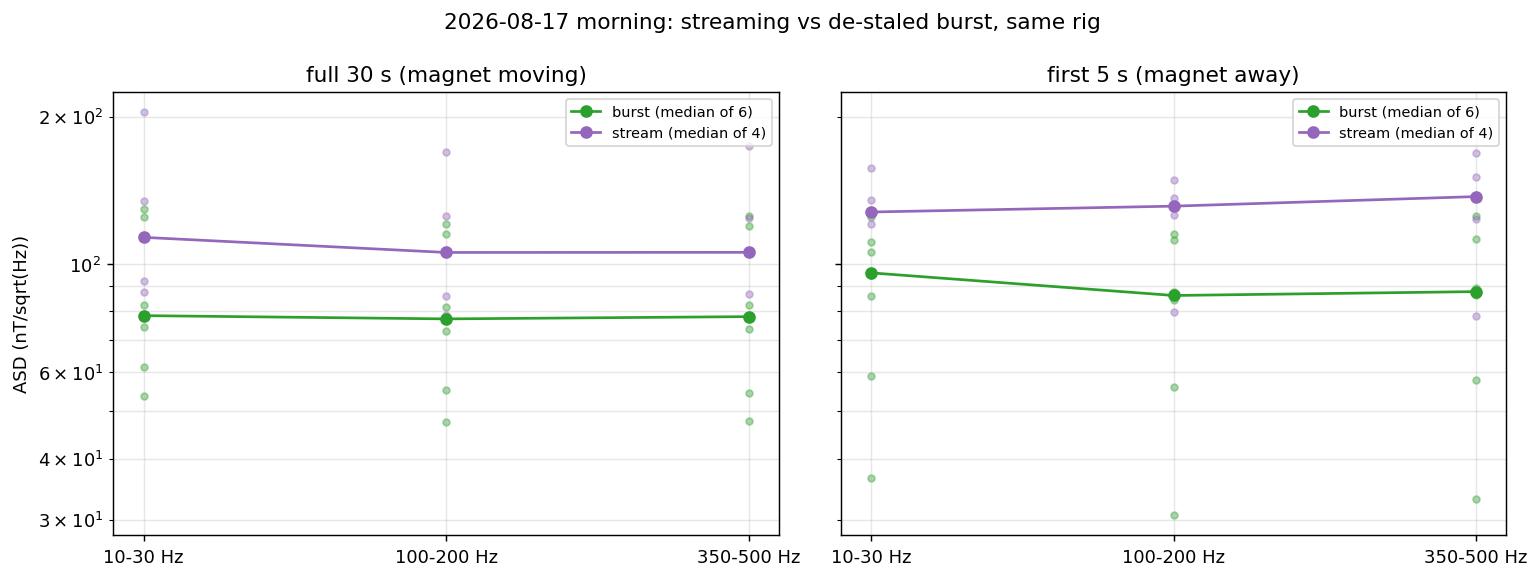
\includegraphics[width=\linewidth]{figures/0817_read_paths.png}
\caption{2026-08-17 morning. Points are individual runs, lines the median. The
run-to-run scatter within each mode is a factor of $\sim$2, which is the main
reason this session cannot replace the interleaved A/B.}
\end{figure}

\begin{keybox}[The excess is real but it is 1.3--1.6\texorpdfstring{$\times$}{x}, not 6\texorpdfstring{$\times$}{x}]
Streaming is still worse than burst, still by a flat factor across the band ---
the signature has not changed. But the size has: \textbf{1.3--1.6$\times$} here
against \textbf{5.3--6.3$\times$} on 08-14. Both windows agree, so it is not the
magnet.

Three things differ between the sessions and none has been isolated: the
photodiode gain change, \co{mw_gain} (this session ran at \num{10500}; the
current notebook default is \num{15000}), and the \co{stream()} configuration
sequence, which was aligned with \co{acquire()}'s on 2026-08-16 --- \emph{after}
the 08-14 data and \emph{before} this session. That last one is the leading
candidate precisely because it was the only difference in the read path, and
this is the first data taken with it.

Do not treat the 6$\times$ figure as current. Do not treat 1.4$\times$ as settled
either: \co{profile\_twopoint\_acquire.py --compare-read-paths} interleaves the
two modes on the same program and is still the measurement that closes this.
\end{keybox}

\subsection{What has been ruled out, with the measurement}

\begin{center}
\small
\begin{tabular}{@{}p{4.0cm}p{7.4cm}l@{}}
\toprule
\hd{Candidate} & \hd{Measurement} & \hd{Verdict} \\
\midrule
Mains pickup & The 60\,Hz comb (8 harmonics) accounts for \textbf{4.5\%} of the
  stream's $\Delta f$ variance & ruled out \\
Slow drift / the PL droop & Below $\sim$10\,Hz is \textbf{2.8\%} of the $\Delta f$
  variance (it is 85\% of the \emph{common-mode} variance, but that cancels) & ruled out \\
Dropped reps & \textbf{0} \co{rep_index} gaps in 125\,000 reps & ruled out \\
Duplicated samples & \textbf{0} duplicate rows in 31\,250 samples & ruled out \\
Packet-boundary artefacts & $\sigma$ at the first 5 rows of a packet is
  \textbf{0.96$\times$} the mid-packet $\sigma$ (30.7 vs 31.8 ADC) & ruled out \\
Buffer overflow as packets fill & The 500-sample first packet is \emph{no noisier}
  than the 205-sample ones & ruled out \\
Torn reads (partial accumulations) & The residual is symmetric, skew \textbf{+0.12},
  kurtosis 1.24. Torn reads would skew strongly low & ruled out \\
\bottomrule
\end{tabular}
\end{center}

A flat, structureless, frequency-independent multiplicative excess is what a
\textbf{read-path} difference looks like, not what a physical disturbance looks
like. Both paths pull from the same accumulated buffer; they differ in how they
configure and drain it.

\subsection{What has been done about it}

\co{stream()}'s configuration sequence now mirrors
\co{NVAveragerProgram.acquire()} step for step. It did not before:

\begin{center}
\small
\begin{tabular}{@{}lll@{}}
\toprule
& \hd{\co{acquire()}} & \hd{\co{stream()}, before 2026-08-16} \\
\midrule
\co{config_all}   & yes & yes \\
\co{start_src}    & yes & yes \\
\co{config_bufs}  & yes & yes, \emph{different order} \\
\co{reload_mem}   & \textbf{yes} & \textbf{missing entirely} \\
\co{start_readout}& yes & yes \\
\bottomrule
\end{tabular}
\end{center}

That is the cheapest candidate to eliminate and it costs nothing if irrelevant.
\co{stream()} also now refuses to reshape a packet whose payload size does not
match its own rep count, which would misalign every subsequent sample and mix the
two parked frequencies --- a failure that would produce exactly this signature and
that was previously invisible.

\begin{openbox}[OPEN --- neither change is verified to fix it]
\textbf{Highest-priority open item.} The test is designed and takes about a minute:
\begin{center}
\co{python scripts/profile_twopoint_acquire.py --compare-read-paths --tau 120 --reps 500}
\end{center}
It alternates \co{acquire(per_rep=True)} and \co{stream()} on the \emph{same
program object}, five times, within seconds. Identical FPGA work; only the read path
differs. It compares raw normalised counts rather than kHz, so it does not depend on
the ODMR calibration still being valid.

\begin{itemize}
  \item ratio $\approx 1.0$ $\Rightarrow$ the $\sim$6$\times$ was the environment
        after all, and streaming needs no caveat;
  \item ratio $\gg 1$ $\Rightarrow$ streaming really is noisier on identical work,
        and it is a software defect. Follow with \co{--stream-scan} to see whether
        it grows with buffer fill.
\end{itemize}
\end{openbox}

\section{An interrupted cell wedges the board, and a kernel restart does not clear it}
\label{sec:wedge}

Found 2026-08-17, when Step~4C hung at its auto-zero \co{acquire()} and \co{Ctrl-C}
produced a traceback ending in \co{sock.recv(size, socket.MSG\_WAITALL)}. Fixed the
same day. It is recorded here because it silently contaminates data rather than
only costing time, and because the recovery is not obvious.

\subsection{The mechanism}

\co{qick}'s \co{poll\_data()} takes a \co{timeout} argument that defaults to
\co{None}, and its board-side body is

\begin{center}
\co{length, data = streamer.data\_queue.get(block=True, timeout=timeout)}
\end{center}

\noindent so with the default it blocks \emph{forever}. \co{qickdawg}'s drain loop
called \co{qd.soc.poll\_data()} with no arguments, so every acquire inherited that
default. The queue is fed by the board's readout worker, which only transfers once
the tProc shot counter advances past a stride. If the counter never advances --- a
program that did not start, a tProc left running by an earlier cell, an abandoned
\co{stream()} generator --- nothing is ever queued and the RPC never replies.

The client then sits in \co{sock.recv(..., MSG\_WAITALL)} waiting for a reply that
is not coming. That is the traceback above, and the four consequences are:

\begin{enumerate}
  \item \textbf{The wait is unbounded.} No timeout, anywhere in the path.
  \item \textbf{\co{Ctrl-C} only unblocks the client.} The board-side Pyro worker
        thread stays blocked in \co{queue.get()} for the life of the daemon.
  \item \textbf{That thread is still a consumer.} When the next run finally queues a
        packet, the abandoned \co{get()} can take it instead of the live caller ---
        so a subsequent run silently loses its first packet.
  \item \textbf{Restarting the notebook kernel does not help}, because the wedged
        thread is on the board, not in the client.
\end{enumerate}

\subsection{Reproduced offline}

Against the real \co{qick.streamer.DataStreamer} driven by a fake board whose shot
counter never advances (\file{scripts/} is not needed; the check is eight lines):

\begin{center}
\begin{tabular}{@{}lll@{}}
\toprule
call & argument & result \\
\midrule
\co{poll\_data()} & \co{timeout=None} (the default) & never returned; killed at 3\,s \\
\co{poll\_data(totaltime=0.1, timeout=1.0)} & finite & returned \co{[]} after 1.01\,s \\
\bottomrule
\end{tabular}
\end{center}

\subsection{The first fix, and why it had to be withdrawn}
\label{sec:boundedpollretraction}

\begin{retractbox}[title=\textbf{Bounding the poll broke two of the three methods. Do not reinstate it.}]
The obvious fix --- pass a finite \co{timeout} so the block becomes a
\co{queue.Empty} --- shipped on 2026-08-17 at 14:23 (commit \co{9832e07}) with
\co{POLL\_TIMEOUT\_S = 1.0}. It was verified against a hand-written mock, never
against the board. Two hours later, on the rig:

\begin{center}
\small
\begin{tabular}{@{}lllp{5.6cm}@{}}
\toprule
\hd{Step} & \hd{Mode} & \hd{reps} & \hd{Result} \\
\midrule
4A & averaged & 35   & worked, \SI{104.5}{\hertz} \\
4B & burst    & 2000 & \co{TimeoutError: acquire() read 0 of 2000 shots and then
                       saw nothing for 10.0 s} \\
4C & stream   & 2000 & hung \emph{anyway}, in \co{Pyro4 socketutil.recvall} \\
\bottomrule
\end{tabular}
\end{center}

Both failures are at the same call --- the dedicated large-reps auto-zero acquire
--- and 4A never makes one, which is why it survived.

The reason a bounded poll is not a safe drop-in is in \co{poll\_data}'s body
(\file{qick/qick.py}):

\begin{center}
\begin{minipage}{0.86\linewidth}\small
\begin{verbatim}
time_end = time.time() + totaltime
while streamer.count < streamer.total_count and time.time() < time_end:
    length, data = streamer.data_queue.get(block=True, timeout=timeout)
    if streamer.stop_flag.is_set() or data is None:
        break            # <-- the packet is DISCARDED, not counted
    streamer.count += length
    new_data.append((length, data))
\end{verbatim}
\end{minipage}
\end{center}

With \co{timeout=None} the \co{get} blocks until a packet exists, so the RPC
always makes forward progress and a slow first stride is simply a wait. With a
finite timeout it returns \co{[]} instead, and the client loop turns that into a
hard failure --- a transient board-side condition becomes a dead run. The
\co{stop\_flag} branch makes it worse: it drops the packet it just took, so a
bounded poll can consume data and report none.
\end{retractbox}

\subsection{What is actually shipped}

\begin{keybox}[title=\textbf{Blocking poll, bounded cleanup, explicit recovery}]
\begin{enumerate}
  \item \textbf{The poll blocks, as qick intends.} \co{POLL\_TIMEOUT\_S = None} is
        the default in \co{NVAveragerProgram}, and both \co{\_drain\_readout()} and
        \co{stream()} read it from there so the two paths cannot drift apart. Set
        it to a float for a diagnostic run and the bounded behaviour --- including
        \co{stream()}'s \co{poll\_timeout\_s} --- comes back.
  \item \textbf{An empty return is an error, not a spin.} Under a blocking poll,
        \co{[]} cannot mean ``the board is slow''; it means the readout ended, or
        somebody else drained the queue. Both loops raise, naming how many shots
        they got. The original code spun on the same condition, hammering the board
        with RPCs; a naive fix would have short-read zeros into the tail of
        \co{d\_buf} instead.
  \item \textbf{Interrupts still clean up} --- this is the half of \co{9832e07}
        worth keeping, and it works fine with a blocking poll, because Pyro raises
        \co{KeyboardInterrupt} inside \co{sock.recv}. The drain loop catches
        \co{BaseException} and \co{stream()} has a \co{finally}, which for a
        generator also runs on \co{GeneratorExit}. Both call \co{\_abort\_readout()}:
        stop the tProc, then stop the readout.
  \item \textbf{Recovery is explicit and staged.} \co{recover()} first stops the
        tProc, stops the readout and \emph{drains the data queue} --- the draining
        is what keeps the next run from picking up leftovers, and it is enough
        after an ordinary \co{Ctrl-C}. Only if the board is still not idle does it
        escalate to \co{DataStreamer.start\_worker()}, which installs fresh queues
        so anything blocked on the old one is orphaned, at the cost of leaking a
        board-side thread. \co{recover(force=True)} goes straight there.
  \item \textbf{\co{ensure\_idle()} reports; it does not act.} It used to call
        \co{recover()} automatically when it found the board busy. Replacing the
        streamer's queues implicitly, at the top of every acquisition cell,
        possibly on a false positive from the probe, is a larger risk than the
        condition it guards. It now prints and returns \co{False}, and Steps 4A/4B/4C
        raise and point at Step 0.
\end{enumerate}
\end{keybox}

\begin{openbox}[title=\textbf{Still open: does the wedge explain the burst replay? Probably not.}]
Consequence 3 above is a mechanism by which one run's packet is delivered to a
\emph{different} run's consumer, which fits the alternating short/long signature.

The 2026-08-17 morning session argues against it. Those runs were taken on a
second computer at commit \co{8fd303f} --- before any of this --- and their stale
fraction is \textbf{50.0--50.8\% across six burst files}
(\file{tables/0817\_burst\_audit.csv}), the same as 08-06 and 08-14. A wedge is an
incident; it should not reproduce at exactly one batch in two, on two machines,
across three sessions. Whatever causes the replay is structural.

Still worth measuring, and free: run a burst now that the poll is blocking again
and read \co{BURST\_STALE\_FRACTION}.
\end{openbox}

\section{Averaged and burst runs used to overwrite each other's filenames}
\label{sec:namecollision}

Step~4A and Step~4B both wrote \co{twopoint\_lockin\_live\_<stamp>.csv}. Nothing was
lost --- the timestamps differ --- but an averaged run and a burst run were
indistinguishable by name, which is why identifying which recorded file was which
mode has repeatedly needed column inspection rather than a glance at the directory.

Fixed 2026-08-17: Step~4A writes \co{twopoint\_lockin\_avg\_*}, Step~4B writes
\co{twopoint\_lockin\_burst\_*}, Step~4C already wrote \co{twopoint\_lockin\_stream\_*}.
\co{find\_live\_csvs()} in \file{analyze\_twopoint\_session.py} accepts all three
prefixes so previously recorded sessions still load unchanged. Files already on disk
keep their \co{\_live\_} names and are still found; only the mode has to be read from
the columns, which \co{detect\_mode()} does anyway.


\section{Post-processing: recovering runs already recorded}
\label{sec:postproc}

Independently of any hardware fix, existing burst files can be made usable. The
pipeline is \co{process_burst()} in \file{twopoint_postprocess.py}, reachable from
the command line as \co{scripts/clean_burst_lockin.py}. It applies, in order:

\begin{enumerate}
  \item \textbf{Stale-batch removal}, by the two tests above. Reports the fraction.
  \item \textbf{Row-0 transient removal} from every batch.
  \item \textbf{Re-timing on the exact cadence} from \S\ref{sec:quantum}, with each
        surviving burst marked as its own \co{segment} so the inter-burst dead time
        is an explicit gap. Nothing is interpolated across it and spectra are
        computed per segment.
  \item \textbf{Differential despiking} --- a causal Hampel filter on
        \co{peak_shift_kHz}.
\end{enumerate}

\paragraph{Order matters.} Staleness is judged on the \emph{unfiltered} frame,
because the batch table reconstructs each batch's start time from its first row;
dropping row 0 first would shift every start by half a sample.

\paragraph{What it cannot do.} The samples lost to the dead time between bursts are
not there, and the genuine single-rep glitches that were double-counted are
\emph{de}-duplicated, not explained. It recovers a correct 3.1\,kHz record from a
6.2\,kHz one; it does not recover 6.2\,kHz.

\subsection{A bug this found: never despike the channels separately}
\label{sec:despikebug}

\begin{keybox}[Per-channel despiking makes the data worse]
The two parked channels are \textbf{0.84--0.97 correlated} through the common-mode
PL. A Hampel filter run on them independently flagged \textbf{30 and 23} samples
with only \textbf{4 in common} --- so most replacements are one-sided, and each
one-sided replacement breaks the cancellation the estimator depends on and
\emph{injects} differential noise.

Measured effect:
\begin{center}
\small
\begin{tabular}{@{}lrrr@{}}
\toprule
& \hd{raw} & \hd{per-channel} & \hd{differential} \\
\midrule
averaged 145321 & 54.6\,kHz & \textcolor{bad}{55.8\,kHz} & \textcolor{good}{\textbf{53.6\,kHz}} \\
stream 145442   & 160.8\,kHz & \textcolor{bad}{175.5\,kHz} & \textcolor{good}{\textbf{155.2\,kHz}} \\
\bottomrule
\end{tabular}
\end{center}

The default is now \co{despike="shift"}, which filters the differential.
Per-channel remains available as \co{despike="channels"} for diagnosing raw-channel
glitches, and prints a warning saying it will usually raise $\sigma$.
\end{keybox}

The live-loop despiker is a separate case and legitimately per-channel: there, the
raw channels must be cleaned \emph{before} the conversion exists. It is off by
default (\co{AVG_DESPIKE_ENABLED = False}).

\chapter{Work log: what has been changed and pushed}
\label{ch:worklog}

Repository: \file{github.com/chalach49266/nv-compact-magnetometer}, branch
\co{main}. All commits below are pushed. The two sessions are separated because the
second one partly retracts the first.

\begin{retractbox}[title=\textbf{Read Round 7 first --- the acquisition path was reverted}]
On 2026-08-18 the acquisition \emph{modules} were reset to revision \co{8fd303f},
the one the second machine takes good data with. Everything Rounds 3, 4 and 6
changed on that path is \textbf{no longer in the code}. The notebooks were kept.
Rounds 1, 2 and 5 stand: measurement, analysis and figure saving, none of which
touch acquisition.
\end{retractbox}

\section{Round 1 --- 2026-08-12, against the 2026-08-06 session}

\begin{center}
\small
\begin{tabular}{@{}llp{8.6cm}@{}}
\toprule
\hd{Commit} & \hd{Scope} & \hd{What it did} \\
\midrule
\co{5ea75ab} & \co{data:} & 2026-08-06 session snapshot (drone sweeps, burst runs,
  17-point integration-time scan). \\
\co{50fe514} & \co{docs:} & The timing \& noise analysis, plus
  \co{analyze_twopoint_session.py} and \co{profile_twopoint_acquire.py}. \\
\co{942d9e8} & \co{perf:} & Corrected the \co{config_all} keyword; $\tau$ 213
  $\rightarrow$ \SI{120}{\micro\second}; added ABBA ordering; append-only CSV writer. \\
\co{6765284} & \co{fix:} & \co{MultipointLockinODMR.stream()} --- the continuous
  streaming path. \\
\co{9eed2e1} & \co{feat:} & \co{clean_burst_lockin.py}, to salvage burst runs already
  recorded. \\
\co{16fd9ba} & \co{docs:} & Changelog, rig checklist, cross-references. \\
\co{f700223} & \co{fix:} & Sensitivity omitted the $\sqrt{\text{reps}}$ factor,
  understating $\eta$ by $\sim$10$\times$. \\
\bottomrule
\end{tabular}
\end{center}

\paragraph{Scorecard on round 1.} Of the four changes intended to improve things:

\begin{center}
\small
\begin{tabular}{@{}p{6.0cm}lp{6.4cm}@{}}
\toprule
\hd{Change} & \hd{Outcome} & \hd{Verdict} \\
\midrule
$\tau$ 213 $\rightarrow$ \SI{120}{\micro\second} & \Partial &
  Took effect and is right for sensitivity, but bought \textbf{no rate} --- the
  premise that $\tau$ set the rate was wrong. \\
\co{config_all} fix + \co{reset_tproc} & \Open &
  Real bug, correctly fixed, but \textbf{did not stop the replay}. \\
\co{stream()} & \Done &
  Works: \textbf{1041.7\,Hz}, gapless. Its noise is a new open defect. \\
Append-only CSV writer & \Done &
  Removed the 25--220\,ms periodic stalls. \\
ABBA ordering & \Open & Implemented, never tested on hardware. \\
\bottomrule
\end{tabular}
\end{center}

\section{Round 2 --- 2026-08-16/17, against the 2026-08-14 session}

\begin{center}
\small
\begin{tabular}{@{}llp{8.2cm}@{}}
\toprule
\hd{Commit} & \hd{Scope} & \hd{What it did} \\
\midrule
\co{a98fd2f} & \co{data:} &
  2026-08-14 session (101\,MB): four averaged runs, one stream run, one burst run
  all at $\tau$=\SI{120}{\micro\second}; a 12-point integration-time sweep
  (1--\SI{213}{\micro\second}, 5 repeats each); an 8-peak reference sweep; a
  multipoint run. Committed \emph{before} any code change, so the analysis has a
  fixed baseline. \\[3pt]
\co{6eb7eb5} & \co{docs:} &
  \textbf{Retraction} of the ``rate is FPGA-bound'' conclusion in the 2026-08-06
  document, with the evidence, plus marking \S4.3's root cause disproved. \\[3pt]
\co{524dbb4} & \co{feat:} &
  \file{twopoint_spectra.py} (365 lines) and \file{twopoint_postprocess.py}
  (790 lines); \co{clean_burst_lockin.py} rewritten to delegate. Found and fixed the
  per-channel despiking bug and the 12\% burst-cadence error. \\[3pt]
\co{6893bcb} & \co{perf:} &
  Corrected rate model (\co{HOST_CALL_S}/\co{HOST_FLOOR_S} replacing
  \co{HOST_OVERHEAD_S}); \co{reps_that_fit()}; \co{measure_host_floor()};
  \co{multipoint_on_stale="drop"}; \co{stream()} sequence aligned with
  \co{acquire()} and packet-size validation. \\[3pt]
\co{8fd303f} & \co{refactor:} &
  Notebook split into Step 4A/5A, 4B/5B, 4C/5C, Step 6. New
  \file{twopoint_runner.py} (236 lines) for the shared plumbing. 1497 lines of
  notebook changed. \\[3pt]
\co{68e95a9} & \co{feat:} &
  Three rig tests: \co{--compare-read-paths}, \co{--stream-scan}, \co{--floor}. \\[3pt]
\co{f1bd0eb} & \co{docs:} &
  The 2026-08-14 methods document, \co{analyze_twopoint_0814.py}, five generated
  tables and three figures; pointer fixes in \co{LOCKIN_ACQUIRE.md} and
  \co{twopoint_lockin_notes.md}. \\
\bottomrule
\end{tabular}
\end{center}

\section{Round 3 --- 2026-08-17, the board wedge}

Triggered by a live failure at the rig rather than by analysis: Step~4C hung at its
auto-zero \co{acquire()}, and \co{Ctrl-C} would not release it. Diagnosed to
\co{poll\_data()}'s \co{timeout=None} default and fixed the same day. Full account in
\S\ref{sec:wedge}; the naming collision in \S\ref{sec:namecollision} was found while
tracing which file each mode had written.

\begin{retractbox}[title=\textbf{Read Round 4 before acting on anything in this section}]
The central change below --- bounding every poll --- was \textbf{withdrawn the same
day}. It broke burst and streaming on first contact with the board.
\S\ref{sec:boundedpollretraction} is the account; \S\ref{sec:round4} is what
replaced it. The interrupt cleanup and the naming split survive unchanged.
\end{retractbox}

\begin{center}
\small
\begin{tabular}{@{}lp{10.4cm}@{}}
\toprule
\hd{Scope} & \hd{What it did} \\
\midrule
\co{fix(qickdawg):} &
  \co{acquire()}'s drain loop extracted to \co{\_drain\_readout()} and bounded: an
  explicit \co{poll\_data} timeout, a no-progress deadline that raises
  \co{TimeoutError}, and a \co{BaseException} handler that stops the tProc and the
  readout before re-raising. Adds \co{POLL\_TOTALTIME\_S}, \co{POLL\_TIMEOUT\_S},
  \co{ACQUIRE\_IDLE\_S}, \co{\_acquire\_timeout\_s()} and \co{\_abort\_readout()}. \\[3pt]
\co{fix(twopoint):} &
  \co{stream()} passes the same explicit timeout --- which is what finally makes its
  own \co{poll\_timeout\_s} reachable --- and wraps its loop in \co{try/finally}, so an
  interrupted or abandoned generator leaves the board idle. Records
  \co{stream\_qc()["aborted"]}. \\[3pt]
\co{feat(twopoint):} &
  \co{MultipointLockinODMR.recover()} and \co{ensure\_idle()}. The pre-flight is wired
  into Steps 4A, 4B and 4C. \\[3pt]
\co{fix(notebook):} &
  Step~4A writes \co{twopoint\_lockin\_avg\_*} and Step~4B \co{twopoint\_lockin\_burst\_*}
  instead of both writing \co{\_live\_}; \co{find\_live\_csvs()} accepts all three
  prefixes. \\
\bottomrule
\end{tabular}
\end{center}

\subsection{Verified offline}

No board was available, so all three paths were exercised against fakes built from
the real \co{qick} sources:

\begin{center}
\small
\begin{tabular}{@{}>{\raggedright\arraybackslash}p{2.4cm}
                  >{\raggedright\arraybackslash}p{6.4cm}
                  >{\raggedright\arraybackslash}p{4.6cm}@{}}
\toprule
\hd{Check} & \hd{What it drives} & \hd{Result} \\
\midrule
Root cause & real \co{DataStreamer}, counter frozen;
  \co{poll\_data()} vs \co{poll\_data(timeout=1.0)} &
  hangs vs returns in 1.01\,s \\[3pt]
Healthy drain & \co{\_drain\_readout()} from the edited file, 50 shots in
  10-shot packets & 50/50, buffer bit-exact \\[3pt]
Stalled tProc & same, board returns nothing &
  \co{TimeoutError} at the budget, board cleaned \\[3pt]
Interrupt & \co{KeyboardInterrupt} mid-drain &
  re-raised, board cleaned \\[3pt]
Stream abort & real \co{stream()} source, consumer breaks after 10 reps &
  \co{finally} ran, \co{aborted=True} \\[3pt]
Stream completion & same, run to 20/20 reps &
  cleaned, \co{aborted=False} \\
\bottomrule
\end{tabular}
\end{center}


\section{Round 4 --- 2026-08-17 evening, undoing Round 3's central change}
\label{sec:round4}

Round 3 shipped at 14:23 and the rig session at 14:25--14:29 showed it had broken
two of the three acquisition methods. The evidence is the notebook's own saved
outputs:

\begin{center}
\small
\begin{tabular}{@{}cllll@{}}
\toprule
\hd{Cell} & \hd{Step} & \hd{exec} & \hd{reps in the failing call} & \hd{Result} \\
\midrule
18 & 4A averaged & 21 & 35   & worked --- 1067 samples, \SI{104.5}{\hertz} \\
22 & 4B burst    & 25 & 2000 & \co{TimeoutError}: read 0 of 2000 shots in \SI{10}{\second} \\
26 & 4C stream   & 27 & 2000 & hung in \co{Pyro4 socketutil.recvall}; released by \co{Ctrl-C} \\
24 & 5B analysis & 47 & ---  & \co{TypeError: ... not 'NoneType'} (collateral) \\
\bottomrule
\end{tabular}
\end{center}

Both real failures are the dedicated large-reps auto-zero \co{acquire()}, which
4A never makes. The comparison that settled it was the 2026-08-17 \emph{morning}
session, taken on a second computer at \co{8fd303f} --- before Round 3 --- which
streamed \num{31250} samples at \SI{1041.7}{\hertz} with zero missing reps, four
times over. Same rig, same board, same day; the only difference was the code.

\begin{center}
\small
\begin{tabular}{@{}lp{10.4cm}@{}}
\toprule
\hd{Scope} & \hd{What it did} \\
\midrule
\co{revert(qickdawg):} &
  \co{POLL\_TIMEOUT\_S} back to \co{None}, restoring qick's blocking
  \co{poll\_data()}. The no-progress deadline is now consulted only when the poll
  is bounded, which it no longer is by default; set the class attribute to a float
  for a diagnostic run. \S\ref{sec:boundedpollretraction} carries the reason at
  length so this is not re-attempted. \\[3pt]
\co{fix(qickdawg):} &
  An empty return under a blocking poll now raises, naming how many shots were
  read. Previously that condition spun on the board with RPCs; the naive
  alternative would short-read zeros into the tail of \co{d\_buf}. \\[3pt]
\co{fix(twopoint):} &
  \co{ensure\_idle()} reports and no longer calls \co{recover()} implicitly.
  \co{recover()} is staged: stop, drain the data queue, and only escalate to
  \co{start\_worker()} if the board is still not idle (\co{force=True} skips
  ahead). Steps 4A/4B/4C raise and point at the new Step~0 instead of continuing
  into a hang. \\[3pt]
\co{fix(twopoint):} &
  \co{stream\_headroom()} read \co{qd.soc['readouts']}, and \co{qd.soc} is a Pyro
  \co{Proxy} --- not subscriptable --- so the check printed an error for the whole
  2026-08-17 session instead of a number. It now uses \co{qd.soccfg}. This is the
  check the multipoint streaming path actually depends on. \\[3pt]
\co{fix(notebook):} &
  \co{twopoint\_postprocess.process(None)} raises a named error saying which run
  cell to re-run; Steps 5A/5B/5C fall back to the newest matching CSV on disk.
  \co{default\_config.mw\_gain} hoisted to a named \co{MW\_GAIN} constant with its
  provenance --- it went \num{10500}$\rightarrow$\num{15000} inside a commit whose
  subject was ``normalise JSON encoding''. \\[3pt]
\co{feat(notebook):} &
  Steps 4S and 5S in \file{Modules/Lockin_module.ipynb}: streaming for the
  multipoint lock-in with its own post-processing and vector reconstruction
  (Ch.~\ref{ch:mpstream}). \\[3pt]
\co{test(scripts):} &
  \file{scripts/test\_drain\_readout.py}, which exercises the drain loop against
  \co{qick}'s \emph{real} \co{poll\_data} rather than a mock --- the gap that let
  Round 3 ship. 17 checks, no board needed. \\[3pt]
\co{docs(scripts):} &
  \file{scripts/analyze\_twopoint\_0817.py} regenerates every 2026-08-17 number in
  this document. \\
\bottomrule
\end{tabular}
\end{center}

\begin{keybox}[The process lesson, which is the expensive one]
Round 3's commit message says ``Verified offline (no board)''. It was --- against a
mock written alongside the fix, which modelled \co{poll\_data} as ``returns
packets, or \co{[]} on timeout''. The real \co{poll\_data} also discards a packet
when \co{stop\_flag} is set, and returns \co{[]} the moment its \SI{100}{\milli\second}
\co{totaltime} expires. Neither behaviour was in the mock, and both matter.

\file{scripts/test\_drain\_readout.py} now extracts \co{poll\_data}'s source from
the installed \co{qick} and executes it, and fails loudly if that extraction stops
matching. A mock of the component you are debugging tests your belief about it,
not it.
\end{keybox}

\begin{openbox}[title=\textbf{Two more traps found while tracing this, both still live}]
\begin{itemize}
  \item \textbf{\co{qickdawg} resolves to the wrong checkout unless the project
        root is first on \co{sys.path}.} It is pip-installed editable from
        \file{\textasciitilde/Documents/PhD/NV Compact Magnetometer/qick-dawg/src},
        which carries none of this project's patches. The notebooks are safe --- cell~0
        inserts \co{PROJECT\_ROOT} at position 0 --- but a bare
        \co{python scripts/foo.py} is not. \file{test\_drain\_readout.py} asserts
        which copy it imported; other scripts do not.
  \item \textbf{The burst replay reproduces on a second machine.} 50.0--50.8\%
        across six 2026-08-17 morning burst files, at \co{8fd303f}. It is not an
        artefact of this laptop, and it is not the wedge (\S\ref{sec:replay}).
\end{itemize}
\end{openbox}

\section{The notebook layout}
\label{sec:notebook}

\file{Modules/Twopoint_Lockin_module.ipynb}, 34 cells. Step 4 used to be a single
26\,kB cell with a \co{LIVE_BURST_MODE} switch, and Step 5 a single generic analysis
cell that treated all three methods alike --- which is wrong in a different way for
each of them.

\begin{center}
\small
\begin{tabular}{@{}clp{8.4cm}@{}}
\toprule
\hd{Cells} & \hd{Section} & \hd{Contents} \\
\midrule
0--5   & setup & project root, \co{MW_GAIN} and \co{default_config} ($\tau$ set
  here), DSA attenuation \\
6--7   & \textbf{Step 0} & board recovery. Skip it on a normal day; run it after
  any interrupted acquisition (\S\ref{sec:wedge}) \\
8--10  & ODMR sweep & the reference sweep \\
11--14 & Step 1a / 1b & pick the peak to track; place the parked pair and build
  \co{TWOPOINT_CALIB} (this is where the slopes and baselines come from) \\
15--18 & Step 2 / 3 & one batch at the two parked frequencies; apply the conversion \\
\midrule
19--20 & \textbf{Step 4A} & averaged acquisition. Measures the host floor, sizes
  \co{reps} to fill it, prints the alias warning. Writes \co{twopoint_lockin_avg_*} \\
21--22 & Step 5A & \co{process_averaged} + ASD, $\sim$15 lines \\
23--24 & \textbf{Step 4B} & burst acquisition, \co{on_stale="drop"}, cadence-based
  timestamps, reports \co{BURST_STALE_FRACTION}. Writes \co{twopoint_lockin_burst_*} \\
25--26 & Step 5B & \co{process_burst} + per-segment ASD \\
27--28 & \textbf{Step 4C} & streaming acquisition, \co{stream_qc()} assertions.
  Writes \co{twopoint_lockin_stream_*} \\
29--30 & Step 5C & \co{process_stream} + ASD, optional mains notch \\
31--32 & Step 6 & post-process \emph{any} saved run; mode detected from the columns;
  side-by-side comparison table \\
33     & Caveats & what the method does and does not measure \\
\bottomrule
\end{tabular}
\end{center}

Each Step 4x opens with a one-RPC \co{ensure_idle()} that raises and points at
Step~0 rather than starting into a board that is not free. Each Step 5x falls back
to the newest run of its own mode on disk when its partner's \co{*_LAST_CSV} is
unset, so a failed acquisition produces a sentence rather than a \co{TypeError}
from inside \co{pathlib}.

Each Step 4x is self-contained --- it builds its own program, primes, auto-zeroes and
writes its own CSV --- with the parameters that change run to run inline, where they
are edited. Each Step 5x reads the run its partner just wrote. The shared mechanical
plumbing (append-only CSV writer, row building, the timing/freshness/calibration
reports, the standard figure) lives in \file{notebook_modules/twopoint_runner.py} so
that 4A and 4B do not carry 150 duplicated lines each.

\section{Round 6 --- 2026-08-18, the shot counter was never cleared}
\label{sec:counter}

\begin{keybox}[One missing line, and it was never in this file]
\co{acquire()} and \co{stream()} arm the board-side readout without first zeroing
the tProc shot counter. qick's own \co{AcquireProgram.start_round()} does it one
line after \co{reload_mem()}:
\begin{quote}\small\ttfamily
soc.reload\_mem()\\
\# make sure count variable is reset to 0\\
soc.clear\_tproc\_counter(addr=self.counter\_addr)
\end{quote}
The vendored \file{qickdawg/nvpulsing/nvaverageprogram.py} reproduces every other
step of that sequence and drops this one.
\end{keybox}

\subsection{What the counter does}

It is tProc \emph{data memory} at \co{counter_addr}, and nothing in the acquire
path resets it: the program only ever increments it, \co{stop_tproc(lazy=True)}
is a documented no-op on tProc v1 (\S\ref{sec:rpc}, stage 1b), and
\co{reload_mem()} reloads the program's own data, not this address. So it carries
the previous run's final value into the next run.

The board-side worker (\file{qick/streamer.py}) then does:

\begin{quote}\small\ttfamily
shots = self.soc.get\_tproc\_counter(addr=counter\_addr)\\
if shots >= min(last\_shots+stride, total\_shots):\\
\ \ \ \ newshots = shots - last\_shots\quad\#\ last\_shots starts at 0\\
\ \ \ \ data = self.soc.get\_accumulated(ch=ch, address=addr,\\
\ \ \ \ \ \ \ \ \ \ \ \ \ \ \ \ \ \ \ \ \ \ \ \ \ \ \ \ \ \ \ \ \ \ \ \ length=newshots*reads\_per\_count)
\end{quote}

With a stale counter that test passes on the worker's \emph{first} look, before
the new program has written anything, and it transfers whatever is sitting in the
accumulated buffer. Two outcomes, depending only on how the stale value compares
to the new run's length:

\begin{center}
\small
\begin{tabular}{@{}lp{9.6cm}@{}}
\toprule
\hd{Stale counter} & \hd{What happens} \\
\midrule
$>$ \co{total_count} &
  One oversized packet. \textbf{This is the 2026-08-18 crash}: a 100-rep priming
  \co{acquire()} inherited 2000 from the preceding auto-zero and raised
  \co{ValueError: could not broadcast input array from shape (4000,2) into shape
  (200,2)} --- $2000\times2$ readouts into a $100\times2$ array. \\[3pt]
$=$ \co{total_count} &
  \textbf{No error at all.} The call returns in milliseconds with the
  \emph{previous} run's contents. \\[3pt]
$<$ \co{total_count} &
  A short head of stale data, then the run proceeds normally. \\
\bottomrule
\end{tabular}
\end{center}

\subsection{Which paths were affected}

\co{reset_tproc=True} routes \co{config_all} through \co{stop_tproc(lazy=False)},
which on tProc v1 is \co{tproc.reset()} + \co{reload_program()} --- and a reset
plausibly zeroes data memory as a side effect. That is why the damage is uneven:

\begin{center}
\small
\begin{tabular}{@{}lcp{6.4cm}@{}}
\toprule
\hd{Call site} & \hd{\co{reset_tproc}} & \hd{Exposure} \\
\midrule
Step 4A, every sample            & default \co{False} & every call after the first inherited the last one's count \\
Step 4B, the burst \co{acquire}  & \textbf{\co{True}} & probably protected by the reset \\
Step 4B/4C priming and auto-zero & default \co{False} & \textbf{where the crash happened} \\
Step 4C \co{stream()}            & n/a                & armed \co{start_readout} directly, never cleared \\
ODMR sweep, Steps 1--3           & default \co{False} & one \co{acquire} per sweep point \\
\bottomrule
\end{tabular}
\end{center}

\begin{openbox}[Do not yet credit this with the burst replay]
It is the obvious suspect for \S\ref{sec:replay} --- ``the call returns in
\SI{13}{\milli\second} instead of \SI{425}{\milli\second} with 95.7\% of its rows
bit-identical to the batch before'' is exactly the middle row of the table above.
But burst mode is the one path that passes \co{reset_tproc=True}, so if the v1
reset does zero the counter, burst was already protected and its replay has
another cause.

The rig settles it in one line, run straight after a burst batch:
\begin{center}\co{qd.soc.get_tproc_counter(addr=1)}\end{center}
Zero means the reset clears it and the replay is something else. Non-zero means
this was the cause all along, and \S\ref{sec:replay} can be closed. Step 0's
\co{recover()} now prints the value for exactly this reason.
\end{openbox}

\subsection{The fix}

\begin{center}
\small
\begin{tabular}{@{}lp{8.8cm}@{}}
\toprule
\hd{Where} & \hd{Change} \\
\midrule
\co{acquire()} & \co{clear_tproc_counter(addr=self.counter_addr)} between
  \co{reload_mem()} and \co{start_readout()}, matching qick. One RPC,
  $\sim$\SI{1}{\milli\second}, on a call that already costs 10--11\,ms. \\[3pt]
\co{stream()} & the same, in the same position. \\[3pt]
\co{_drain_readout()} & an oversized packet now raises a named \co{RuntimeError}
  that says the counter did not start at zero, instead of letting numpy raise
  \co{could not broadcast}, which names neither cause nor fix. \\[3pt]
\co{_abort_readout()} & clears it on the way out, so an interrupted cell does not
  hand a poisoned counter to whatever runs next. \\[3pt]
\co{recover()} & reads the counter, prints it, clears it. \\
\bottomrule
\end{tabular}
\end{center}

\textbf{No notebook cell changed.} Every acquisition in both notebooks goes
through \co{acquire()} or \co{stream()}; the vendored qickdawg has exactly one
\co{start_readout} call site and \co{stream()} is the other, and every
\co{LockinODMR}-style subclass delegates to \co{NVAveragerProgram.acquire} via
\co{super()}.

\subsection{Verified}

\file{scripts/test_shot_counter.py}, 21 checks. It drives qick's \emph{real}
\co{DataStreamer._run_readout} against a fake board whose counter persists between
runs and whose program ramps the counter rather than completing instantly --- the
arithmetic under test lives in that worker, so a mock of the worker would prove
nothing. It reproduces the exact reported shapes, \co{(4000,2)} into
\co{(200,2)}, and shows the clear removes them; shows the equal-counter case
completing silently with data read before the program produced it; and confirms
the call is present in the shipped \co{acquire()}, \co{stream()},
\co{_abort_readout()} and \co{recover()}, in the right order relative to
\co{reload_mem} and \co{start_readout}.

\section{Round 7 --- 2026-08-18, revert the acquisition path to \texorpdfstring{\co{8fd303f}}{8fd303f}}
\label{sec:revert}

Three rounds of changes to the acquisition path each fixed something real and each
left the rig worse than it found it. On 2026-08-18 the operator reported that
streaming still did not run and that averaged mode had fallen to \SI{48}{\hertz},
against the 87--105\,Hz it had held all week, and asked for the path to be made
identical to the revision on the second machine.

\begin{center}
\small
\begin{tabular}{@{}llp{6.0cm}@{}}
\toprule
\hd{File} & \hd{State} & \hd{Why} \\
\midrule
\file{qickdawg/nvpulsing/nvaverageprogram.py} & \textbf{byte-identical to \co{8fd303f}} & the acquire loop and the poll \\
\file{notebook_modules/multipoint_lockin_program.py} & \textbf{byte-identical to \co{8fd303f}} & \co{stream()}, the timing model \\
\emph{all 35} \file{qickdawg/*.py} & \textbf{identical} & nothing else on the path drifted \\
\midrule
\file{Modules/*.ipynb} & \textbf{kept} & the revert is the acquisition \emph{modules}; the notebooks keep Step 0, the \co{_avg_}/\co{_burst_}/\co{_stream_} names, \co{mw_gain = 15000}, the newest-run fallbacks, Steps 4S/5S and figure saving \\
\file{notebook_modules/twopoint_postprocess.py} & kept & post-processing only; never on the acquire path \\
\bottomrule
\end{tabular}
\end{center}

The only notebook edit the revert forced: Step 0 and the three pre-flight guards
called \co{recover()} and \co{ensure_idle()}, which live in the acquisition module
and went away with it. Both are now written inline against the raw \co{QickSoc}
proxy --- \co{stop_tproc}, \co{streamer.stop_readout}, \co{poll_data(totaltime=-1)},
\co{streamer.readout_running} --- all plain remote methods qick itself exposes. So
the notebook keeps the escape hatch and is independent of which module revision is
loaded. The guard also downgraded from fatal to a warning on probe failure: a
board-state probe must never be able to stop a run.

\subsection{What went away with it}

\begin{center}
\small
\begin{tabular}{@{}lp{8.6cm}@{}}
\toprule
\hd{Gone from the modules} & \hd{Consequence} \\
\midrule
\co{POLL_TIMEOUT_S}, \co{_drain_readout} & the poll is qick's plain
  \co{poll_data()} again --- blocking, which is the behaviour that worked. \\
\co{_abort_readout()} & an interrupted cell no longer stops the tProc on the way
  out. After a Ctrl-C mid-readout, run Step 0; if it still reports busy, restart
  the board's Pyro server. A kernel restart will not clear it. \\
\co{ensure_idle()}, \co{recover()} & reimplemented in the notebook instead, as
  above. \\
\co{clear_tproc_counter()} & the stale-counter behaviour of \S\ref{sec:counter} is
  live again --- see the box below. \\
\bottomrule
\end{tabular}
\end{center}

The hardware operating point is \emph{unchanged}: \co{mw_gain = 15000},
$\tau = \SI{120}{\micro\second}$, \co{AVG_REPS_PER_BATCH = None},
\co{BURST_REPS = 500}, \co{STREAM_TARGET_HZ = 1000}. Those live in the notebook,
not in the reverted modules.

\begin{openbox}[The stale shot counter is real and is now unfixed]
\S\ref{sec:counter} is not retracted --- the mechanism was reproduced against
qick's own \co{DataStreamer._run_readout}, and \co{8fd303f} is missing the same
call qick makes. It is an open defect of the reverted revision, and it is the
leading candidate for the burst replay of \S\ref{sec:replay}.

\file{scripts/test_shot_counter.py} is kept for that reason, scoped down to the
mechanism: 13 checks, all passing, none of them asserting anything about the
shipped code. If the fix is revisited, that test is the check it needs to pass.
\end{openbox}

\subsection{The lesson this round is actually about}

Every one of Rounds 3, 4 and 6 was reasoned from the source, verified offline
against a test, and shipped --- and each one changed the rate or broke a mode on
first contact with the rig. Round 3 was verified against a mock and broke burst
and streaming. Round 6 was verified against qick's real worker thread and, whatever
else it did, coincided with averaged mode falling to \SI{48}{\hertz}.

Offline verification says the code does what you think. It says nothing about
whether what you think is worth doing. \textbf{On this rig, the acquisition path
changes one thing at a time, with a before-and-after run on the bench, or it does
not change.}

\begin{center}
\small
\begin{tabular}{@{}lrl@{}}
\toprule
\hd{Session} & \hd{Averaged rate} & \hd{Path revision} \\
\midrule
2026-08-14 & 86.8--88.8\,Hz & \co{8fd303f} lineage \\
2026-08-17 morning \emph{(other machine)} & --- & \co{8fd303f} \\
2026-08-17 afternoon & 104.5\,Hz & \co{9832e07} (burst + stream broken) \\
2026-08-18 & \textbf{48\,Hz} & Round 6 \\
2026-08-18, after this revert & \emph{to be measured} & \co{8fd303f} \\
\bottomrule
\end{tabular}
\end{center}

The last row is the first thing to fill in at the rig.

\section{Round 5 --- 2026-08-18, every figure goes to disk}
\label{sec:autosave}

Neither notebook wrote a single PNG. Every plot lived only in cell output, which
"Restart \& Clear Outputs" discards and which cannot be opened next to the CSV it
describes. The \co{*_result.png}/\co{*_fft.png} pairs already sitting in
\file{data/results/} were produced by a separate tool on the acquisition machine,
not by these notebooks --- nothing in this repository wrote them.

\subsection{\texorpdfstring{\co{notebook_modules/figure_autosave.py}}{figure\_autosave.py}}

Saving is automatic rather than a \co{savefig} line per plot, because there are
twenty-three plotting sites across the two notebooks and adding a line to each
guarantees the twenty-fourth is forgotten.

The module hooks the two moments at which the inline backend destroys a figure:

\begin{center}
\small
\begin{tabular}{@{}lp{9.2cm}@{}}
\toprule
\hd{Hook} & \hd{What it catches} \\
\midrule
\co{post_execute} callback &
  Figures a cell drew but never explicitly showed. It must run \emph{before}
  matplotlib-inline's \co{flush_figures}, which displays and then closes
  everything; IPython fires \co{post_execute} in registration order, so
  \co{enable()} registers its own callback and then re-registers
  \co{flush_figures} to move it to the back of the queue. \\[3pt]
wrapper around \co{pyplot.show} &
  Figures closed mid-cell. \co{show()} on this backend closes what it displays,
  and \co{twopoint_runner.plot_run}, \co{TwoPointResult.figure(show=True)} and the
  live loops in \file{Lockin_module.ipynb} all call it. \\
\bottomrule
\end{tabular}
\end{center}

Both funnel into \co{capture()}, and the ``already written'' marker lives on the
figure object, so the two hooks cannot duplicate each other's work.

\subsection{Naming}

\co{set_run(csv, tag=...)} points the module at a run: the PNGs take the CSV's
stem and land in the CSV's own folder. The numbering restarts on every
\co{set_run}, so \textbf{re-running a cell overwrites that cell's own PNGs}
instead of accumulating copies.

\begin{center}
\small
\begin{tabular}{@{}ll@{}}
\toprule
\hd{Cell} & \hd{Writes} \\
\midrule
Step 4A/4B/4C \co{set_run(AVG_CSV, tag="run")} & \co{twopoint_lockin_avg_<ts>_run_result.png} \\
Step 5A/5B/5C \co{set_run(A5_CSV)} & \co{twopoint_lockin_avg_<ts>_result.png} \\
 & \co{twopoint_lockin_avg_<ts>_fft.png} \\
\bottomrule
\end{tabular}
\end{center}

A figure is classified \co{_fft} only when \emph{all} of its axes are log--log
spectra. That matters here: the three-panel figure from
\co{TwoPointResult.figure()} carries an ASD as its last panel, and must not claim
the \co{_fft} name from the standalone spectrum figure of the same run. A cell can
override the classification entirely with \co{fig.set_label("droop")}, giving
\co{<stem>_droop.png}.

\subsection{\texorpdfstring{\co{TwoPointResult.spectrum_figure()}}{spectrum\_figure()}}

Added so that every two-point run gets a real \co{_fft.png} rather than only the
ASD panel buried at a third height inside \co{figure()}. Full width, with the
white floor, $\eta$ from $\sigma$, and every line above 2$\times$ the floor
annotated with its excess. Steps 5A/5B/5C call it after \co{figure()}.

\subsection{Verified}

\begin{itemize}
  \item \file{scripts/test_figure_autosave.py} --- 18 checks, driven through a
        real \co{InteractiveShell} with \co{\%matplotlib inline} rather than a
        mock, because hook ordering against \co{flush_figures} is the whole
        mechanism. Confirms the ordering explicitly, and covers the unshown-figure
        path, the \co{plt.show()} path, the mixed-figure classification, tags,
        overwrite-on-rerun, empty figures, \co{disable()}/re-\co{enable()} and the
        label override.
  \item \file{scripts/test_notebook_figure_saving.py} --- runs Step 5B and Step 5C
        \emph{out of the \co{.ipynb} files} against scratch copies of the
        2026-08-17 runs, and checks both PNGs appear beside the CSV and that a
        second run overwrites them. 6 checks.
  \item A static pass over both notebooks asserts every cell that draws calls
        \co{set_run} \emph{before} its first plot. That caught one cell where the
        call had landed after the plots and would have filed them under the
        previous run's name.
\end{itemize}

\begin{openbox}[The live loops write one figure, not a movie]
\file{Lockin_module.ipynb} Steps 4 and 4B redraw a single figure in place while
the run proceeds. What reaches disk is that figure's \emph{final} state, which is
the whole run --- not a frame per update. Step 4BN and Step 4S are headless and
draw once at the end, so they are unaffected.

There is also no \co{_fft.png} for the multipoint live cells: their time base is
the host loop period, not a cadence, so an ASD computed on it would put a
frequency scale on jitter. The streamed Step 5S has a real cadence and does
produce one.
\end{openbox}

\section{The code, file by file}
\label{sec:filemap}

\begin{center}
\small
\begin{longtable}{@{}p{5.0cm}p{2.0cm}p{7.2cm}@{}}
\toprule
\hd{File} & \hd{State} & \hd{Role} \\
\midrule
\endhead
\multicolumn{3}{@{}l}{\emph{Acquisition}} \\
\file{notebook_modules/} \file{multipoint_lockin_program.py} & modified &
  The FPGA program, all three read paths, the timing model, the freshness guard. \\
\file{qickdawg/nvpulsing/} \file{nvaverageprogram.py} & modified &
  Vendored; the \co{config_all} fix and \co{reset_tproc} plumbing. \\
\file{Modules/} \file{Twopoint_Lockin_module.ipynb} & restructured &
  32 cells: setup, ODMR, Steps 1--3, then 4A/5A, 4B/5B, 4C/5C, 6. \\
\midrule
\multicolumn{3}{@{}l}{\emph{Analysis (new)}} \\
\file{notebook_modules/} \file{twopoint_spectra.py} & \textbf{new} &
  Every FFT. One-sided PSD, $\eta=\sigma\sqrt{2\Delta t}$, mains-line finder,
  alias report, comb notch. Verified against Parseval. \\
\file{notebook_modules/} \file{twopoint_postprocess.py} & \textbf{new} &
  One pipeline per mode + mode detection + exact readout-quantum recovery + CLI. \\
\file{notebook_modules/} \file{twopoint_runner.py} & \textbf{new} &
  Shared acquisition plumbing: append-only CSV, row building, the three reports,
  the standard figure. \\
\file{notebook_modules/burst_qc.py} & reused &
  Batch table, stale masks, retiming, segment PSD, block averaging. \\
\file{notebook_modules/} \file{spike_rejection.py} & reused &
  \co{HampelDespiker}. \\
\midrule
\multicolumn{3}{@{}l}{\emph{Scripts}} \\
\file{scripts/} \file{analyze_twopoint_0814.py} & \textbf{new} &
  Regenerates every number and figure in this document. \\
\file{scripts/} \file{profile_twopoint_acquire.py} & modified &
  Static signature check + per-RPC timing + the three rig tests. \\
\file{scripts/} \file{clean_burst_lockin.py} & rewritten &
  Burst CLI, now delegating to \co{twopoint_postprocess}. \\
\file{scripts/} \file{analyze_twopoint_session.py} & unchanged &
  The 2026-08-06 analysis; still regenerates that document. \\
\midrule
\multicolumn{3}{@{}l}{\emph{Documents}} \\
\file{docs/twopoint_master_reference/} & \textbf{new} & This document. \\
\file{docs/} \file{2026-08-14_twopoint_methods/} & new & Markdown source + generated tables/figures. \\
\file{docs/} \file{2026-08-06_twopoint_timing/} & annotated & The earlier analysis, with corrections marked in place. \\
\file{docs/LOCKIN_ACQUIRE.md} & pointer fixed & Repeated the retracted 1.6\,ms figure. \\
\file{docs/} \file{twopoint_lockin_notes.md} & pointer fixed & Same. \\
\bottomrule
\end{longtable}
\end{center}

\section{Wiki}

The synthesis is filed in the Obsidian vault at \file{NV Project/}.

\begin{itemize}
  \item \textbf{New page:} \file{wiki/sources/twopoint_three_modes_2026_08_14.md}
  \item \textbf{Correction banner:} \file{wiki/sources/twopoint_timing_and_burst_defect.md}
  \item \textbf{Updated:} \file{wiki/experiments/lockin_tracking.md} (new
        ``August 14--17'' section, and the August 6--12 one partly retracted);
        \file{wiki/concepts/sensitivity.md} (three new rows, plus a warning that the
        two-point noise does not average down);
        \file{wiki/questions/open_questions.md} (three questions answered, four new
        ones with pass criteria); \file{wiki/overview.md} (status table and the
        ``Where We Stand'' list); \file{index.md} (routing).
  \item \textbf{Log entry:} \file{log.md}, dated 2026-08-17.
\end{itemize}

\emph{Not} committed to git: the vault sits inside the home-directory repository,
which contains unrelated and sensitive untracked files. The files are on disk and
sync through OneDrive.


\chapter{What still needs to be done}
\label{ch:todo}

\section{Rig checks, in priority order}
\label{sec:rigchecks}

Everything here needs the RFSoC at 192.168.0.103, reachable only from the Windows
rig machine. Each has a pass criterion.

\begin{center}
\small
\begin{longtable}{@{}p{0.7cm}p{4.6cm}p{4.4cm}p{4.6cm}@{}}
\toprule
\hd{\#} & \hd{Check} & \hd{Command} & \hd{Pass criterion} \\
\midrule
\endhead
S0 & \textbf{Does the wedge fix close the burst replay?} Now the cheapest
  decisive test, because \S\ref{sec:wedge} gives \S\ref{sec:replay} its first
  mechanism since \co{reset_tproc} was eliminated. \emph{Do this first.}
  $\sim$1\,min. &
  Run Step~4B for 30\,s and read \co{BURST_STALE_FRACTION}. &
  \textbf{0\%} $\Rightarrow$ the replay was the wedge and both defects close.
  Still $\sim$\textbf{50\%} $\Rightarrow$ they are independent; S1 next. \\[3pt]
S1 & \textbf{Burst vs stream, interleaved.} Decides whether the $\sim$6$\times$
  streaming excess is the read path or the room. \emph{Do this first.} $\sim$1\,min. &
  \co{profile_twopoint_acquire.py --compare-read-paths --tau 120 --reps 500} &
  ASD ratio within \textbf{1.25$\times$} $\Rightarrow$ environment. Well above
  $\Rightarrow$ software defect. \\[3pt]
S2 & Does the streaming excess grow with run length (buffer fill)? &
  \co{profile_twopoint_acquire.py --stream-scan} &
  Floor at 125\,k reps within \textbf{1.3$\times$} of the floor at 2\,k reps. \\[3pt]
S3 & Confirm the per-call floor and the flat rate. &
  \co{profile_twopoint_acquire.py --floor --tau 120 --reps 1 4 10 23 42 100} &
  Fastest call \textbf{9--11.5\,ms} with a \co{reps=1} probe; period flat to
  \textbf{15\%} across reps whose FPGA work fits under it. \\[3pt]
S4 & \textbf{Fill in \S\ref{sec:rpc}} --- the per-RPC split, the one structural gap
  in this document. &
  \co{profile_twopoint_acquire.py --ip 192.168.0.103} &
  A time for each of stages 1--7. No pass/fail; this is a measurement that has never
  been made. \\[3pt]
S5 & Free averaging. 30\,s Step 4A with \co{AVG_REPS_PER_BATCH = None}. &
  Notebook Step 4A &
  Still $\sim$88\,Hz \emph{and} $\sigma(\Delta f)\le$ \textbf{54.6\,kHz}. Given
  \S\ref{sec:notshot}, expect less than the naive 2$\times$. \\[3pt]
S6 & \textbf{The per-acquire noise term.} Interleave averaged runs at reps =
  10 / 23 / 42 within one sitting. &
  Notebook Step 4A, three configs, alternating &
  Does $\sigma$ fall as $1/\sqrt{\text{reps}}$? If not, the term is per-call --- then
  test whether it tracks the idle gap by varying \co{SAVE_EVERY_SEC} or inserting a
  deliberate sleep. \\[3pt]
S7 & ABBA A/B at fixed $\tau$ and equal averaging (\co{"forward"} 46 reps vs
  \co{"abba"} 23 reps), interleaved. &
  Notebook Step 4A, two configs &
  Report the change in $\sigma(\Delta f)$. Any reduction is free. \\[3pt]
S8 & Honest burst rate with the drop policy. 10\,s Step 4B. &
  Notebook Step 4B, \co{BURST_ON_STALE="drop"} &
  Step 5B reports \textbf{\co{n_stale_batches} = 0} on the file Step 4B just wrote,
  and \co{BURST_STALE_FRACTION} is printed. \\[3pt]
S9 & Instrument the replay. Print the shot counter and queue depth before/after each
  \co{start_readout} during a burst run. &
  needs a small patch to \co{acquire()} &
  Discriminates the three candidate mechanisms in \S\ref{sec:replay}. \\
\bottomrule
\end{longtable}
\end{center}

\section{Software backlog}

\begin{center}
\small
\begin{tabular}{@{}p{5.4cm}lp{7.2cm}@{}}
\toprule
\hd{Item} & \hd{Priority} & \hd{Why} \\
\midrule
Periodic re-zero during a streaming run & high &
  The 25\% PL droop (\S\ref{sec:droop}) walks the operating point off the
  calibrated flank over 30\,s. Currently only detrended in post. \\
Root-cause the burst replay & high &
  Would recover $\sim$15\% of burst rate and remove the need for the drop policy. \\
Real-time mains notch in the acquisition path & medium &
  The current notch is offline, non-causal, and assumes stationarity. At $\ge$1\,kHz a
  causal notch is feasible and the line is 10$\times$ the floor. \\
Fold the multipoint notebook onto the same modules & medium &
  \file{twopoint_spectra.py} and \file{twopoint_postprocess.py} are mode-generic;
  the multipoint path still has its own analysis code. \\
Calibrated field reference & medium &
  Every $\eta$ here is a readout-chain figure (\S\ref{sec:notaclaim}). A known
  applied field would turn them into system claims. \\
\co{remove_offset} is documented but not implemented & low &
  \co{NVAveragerProgram.acquire()} accepts the argument and never uses it. Harmless
  today (both paths are consistent) but a latent trap. \\
Allan deviation on the long runs & low &
  Needed for the drift/averaging-time story; the June time-integration data exists
  but has not been analysed drift-aware. \\
\bottomrule
\end{tabular}
\end{center}

\section{Recommended operating point today}

\begin{keybox}[Until S1 resolves the streaming question]
\begin{description}[leftmargin=1.4em,style=nextline]
  \item[For best sensitivity --- Method B, burst.] $\tau=\SI{120}{\micro\second}$,
  \co{BURST_REPS = 500}, \co{BURST_ON_STALE = "drop"}. 38\,\etaunit\ at an effective
  3.1\,kHz. Accept the $\sim$15\,ms gap every 135\,ms.
  \item[For a continuous trace --- Method C, streaming.] $\tau=\SI{120}{\micro\second}$,
  \co{STREAM_TARGET_HZ = 1000}. 1041.7\,Hz, gapless, exact timestamps, but
  $\sim$6$\times$ the noise until \S\ref{sec:streamnoise} is closed.
  \item[For slow work and sanity checks --- Method A, averaged.]
  $\tau=\SI{120}{\micro\second}$, \co{AVG_REPS_PER_BATCH = None} so the call floor is
  filled. $\sim$88\,Hz, no open defects --- but remember 60\,Hz is aliased into the
  band here.
\end{description}
\end{keybox}


\chapter{Corrections register}
\label{ch:retractions}

Every claim from an earlier document that this one contradicts, in one place.

\begin{center}
\small
\begin{longtable}{@{}p{3.2cm}p{4.6cm}p{4.6cm}p{2.4cm}@{}}
\toprule
\hd{Source} & \hd{Earlier claim} & \hd{Current position} & \hd{Evidence} \\
\midrule
\endhead
2026-08-06 doc \S1, \S2 &
  ``The rate is FPGA-bound, not host-bound''; host round-trip $\sim$1.6\,ms &
  \textbf{Retracted.} Host-bound, $\sim$10--11.4\,ms per call; the FPGA runs
  underneath it &
  \S\ref{sec:floorevidence} \\[3pt]
2026-08-06 doc \S2.6 &
  $\tau$ is ``the main lever''; \co{reps} trades against rate one for one &
  \textbf{Both backwards.} Neither affects the rate below the floor; \co{reps} is a
  free \emph{sensitivity} lever &
  \S\ref{sec:knobs} \\[3pt]
2026-08-06 doc \S2.4 &
  ``Host round-trip 1.60\,ms (14.1\%)'' as a budget row &
  That was a \emph{residual} under an assumed serial model, not a measurement &
  \S\ref{sec:floorevidence} \\[3pt]
2026-08-06 doc \S4.3 &
  \co{config_all} / never-stopped tProc is the root cause of the burst replay &
  \textbf{Disproved.} The fix was applied and 49.9\% still replayed &
  \S\ref{sec:replay} \\[3pt]
2026-08-06 doc \S3.2 &
  ``No 60\,Hz line, no discrete tones'' &
  The line is there and is 10$\times$ the floor; at 87.5\,Hz it is \emph{aliased} to
  $\sim$28\,Hz and the burst runs that could have resolved it were half replays &
  \S\ref{sec:alias} \\[3pt]
2026-08-06 doc, 1st draft &
  $\eta \approx 19$\,\etaunit\ per rep &
  185\,\etaunit. The draft paired a reps-averaged $\sigma$ with a single-rep time,
  omitting $\sqrt{\text{reps}}\approx 10$ &
  \S\ref{sec:conventions} \\[3pt]
2026-08-06 doc, $\eta$ convention &
  $\eta = \sigma_B\sqrt{\Delta t}$ &
  $\eta = \sigma_B\sqrt{2\Delta t}$, matching what the notebook prints; a
  $\sqrt{2}$ difference &
  \S\ref{sec:conventions} \\[3pt]
2026-08-14 doc, 1st draft &
  Streaming excess is ``4.2$\times$'' &
  5.3--6.3$\times$. The 4.2 used the \emph{raw} burst floor; the cleaned floor is
  38.6 rather than 55\,\etaunit &
  \S\ref{sec:streamnoise} \\[3pt]
Notebook Step 4 comment, pre-2026-08-12 &
  ``$\sim$10\,ms of fixed host overhead, FPGA work that fits inside it is FREE'' &
  \textbf{Substantially correct}, and wrongly ``corrected'' on 2026-08-12. Restored &
  \S\ref{sec:model} \\[3pt]
\co{time_per_rep()}, pre-2026-08-12 &
  $n_\text{slots}\times(\tau + 2\,t_\text{relax})$ &
  $n_\text{slots}\times\tau$; the relax windows are absorbed &
  \S\ref{sec:asm} \\[3pt]
Burst cadence, pre-2026-08-16 &
  From \co{acq_seconds/n_samples}: \SI{269}{\micro\second} &
  \SI{240.0}{\micro\second} exactly, from the readout quantum. The old value
  included the host share &
  \S\ref{sec:quantum} \\[3pt]
Despiking, pre-2026-08-16 &
  Filter the two parked channels independently &
  Filter the \emph{differential}. Per-channel raises $\sigma$ &
  \S\ref{sec:despikebug} \\
\bottomrule
\end{longtable}
\end{center}

\begin{keybox}[The methodological lesson]
Four of the twelve rows above come from the same mistake: \textbf{fitting a model
with $n$ free parameters to data taken at one operating point}. The 2026-08-06
session ran at a single $(\tau, \text{reps})$, and every timing conclusion drawn
from it was under-determined --- the serial-versus-overlapped question simply cannot
be answered from one point, however carefully the residuals are computed.

The 2026-08-14 session settled it in an afternoon purely by varying two knobs. Any
future timing claim should span at least three operating points before it is
written down.
\end{keybox}


\chapter{Reproducing everything}

\section{Offline, no hardware}

\begin{quote}\small\ttfamily
\# every number and figure in this document\\
python scripts/analyze\_twopoint\_0814.py\\[4pt]
\# post-process any run; the mode is detected from the columns\\
python -m twopoint\_postprocess <csv> [-{}-outdir DIR] [-{}-notch-mains]\\[4pt]
\# burst-specific CLI with the original flags\\
python scripts/clean\_burst\_lockin.py <live\_csv> -{}-outdir analysis/\\[4pt]
\# the 2026-08-06 analysis, unchanged\\
python scripts/analyze\_twopoint\_session.py\\[4pt]
\# static check of the config\_all signature\\
python scripts/profile\_twopoint\_acquire.py -{}-check-only\\[4pt]
\# rebuild this document\\
cd docs/twopoint\_master\_reference \&\& latexmk -pdf TWOPOINT\_MASTER\_REFERENCE.tex
\end{quote}

\section{On the rig}

\begin{quote}\small\ttfamily
python scripts/profile\_twopoint\_acquire.py -{}-floor -{}-tau 120\\
python scripts/profile\_twopoint\_acquire.py -{}-compare-read-paths -{}-tau 120 -{}-reps 500\\
python scripts/profile\_twopoint\_acquire.py -{}-stream-scan\\
python scripts/profile\_twopoint\_acquire.py -{}-ip 192.168.0.103\\
\hspace*{2em}\# the full per-RPC profile (fills section~\ref{sec:rpc})
\end{quote}

\section{Data used by this document}

\begin{center}
\small
\begin{tabular}{@{}p{6.4cm}p{8.0cm}@{}}
\toprule
\hd{Path} & \hd{Contents} \\
\midrule
\file{data/results/} \file{081426 (Sensitivity increase update)/} &
  2026-08-14: 4 averaged + 1 stream + 1 burst two-point run, all at
  $\tau$=\SI{120}{\micro\second}; 12-point integration sweep; 8-peak reference sweep;
  multipoint run. 101\,MB. \\
\file{data/twopoint_lockin/08062026/} &
  2026-08-06: drone sweeps, 4 burst runs, 12 averaged runs, 17-point integration
  sweep (92 ODMR sweeps). \\
\file{docs/2026-08-14_twopoint_methods/} \file{tables/} &
  Generated: \co{timing.csv}, \co{mode_budgets.csv}, \co{modes.csv},
  \co{read_path.csv}, \co{per_rep_noise.csv}, \co{spectra.csv}. \\
\bottomrule
\end{tabular}
\end{center}


\end{document}
